\documentclass[12pt, twoside]{article}
%\usepackage[hmargin=1.25in, vmargin=1.1in]{geometry}
\usepackage{geometry}

\usepackage[utf8]{inputenc}
\usepackage[T1]{fontenc}
\usepackage[english]{babel}
\usepackage{pdfpages}
\usepackage{listings}
\usepackage{color}
\usepackage{graphicx}
\usepackage{float}
\usepackage{hyperref}
\usepackage{url}
\usepackage{upquote}
\usepackage{lastpage}
\usepackage{fancyhdr}
\pagestyle{fancy}
\usepackage{longtable}
\usepackage{tabu}
\usepackage{rotating}
\usepackage[strings]{underscore}
\usepackage[nottoc,numbib]{tocbibind}
\usepackage{float}
\usepackage[toc,page]{appendix}
\restylefloat{table}

\graphicspath{ {images/} }

\newcommand{\helv}{\fontfamily{phv}\fontseries{b}\fontsize{9}{11}\selectfont}

%--------------- Variables à modifier à chaque rendu ---------------
\title{Report}
\newcommand{\daterendu}{09/08/2019}
%-------------------------------------------------------------------

\makeatletter\let\Title\@title\makeatother

% Décommenter pour commencer les chapitres à 0
%\setcounter{section}{-1}

\begin{document}

\begin{titlepage}

\newcommand{\HRule}{\rule{\linewidth}{0.5mm}} % Defines a new command for the horizontal lines, change thickness here

\center % Center everything on the page



\includegraphics[width=0.8\textwidth]{logo_HEIA.jpg}

\includegraphics[width=0.3\textwidth]{logo_LBNL.png}\\[1.1cm]
\textsc{\Large Bachelor thesis \\ [0.3cm]
\large Year 2018-2019 }\\ [2.0cm]


\textsc{
\bfseries \LARGE Machine learning for noise reduction in images of old audio records}\\ [1.0cm]


\HRule \\[0.5cm]
{ \huge \bfseries \Title }\\ 
\HRule \\[1.2cm]

\Large
Benoit \textsc{Ruffray}\\[1.0cm] 

{\large Date : \daterendu}\\[1.3cm] 

\begin{flushleft}
\large External supervisor: Haber~Carl
\end{flushleft}
\begin{flushleft}
	\large Internal supervisors: Bapst~Frédéric / Hennebert~Jean
\end{flushleft}
\begin{flushleft}
\large Consultants: Cornell~Earl / Nachman~Benjamin
\end{flushleft}

\end{titlepage}
\pagenumbering{Roman}

\renewcommand{\headrulewidth}{1pt}
\fancyhead[L]{\helv ML-for-NR}
\fancyhead[C]{\helv 2018-2019}
\fancyhead[R]{\helv \Title }

\renewcommand{\footrulewidth}{1pt}
\fancyfoot[C]{\helv Table of contents \thepage{}}

\setcounter{page}{1}

\begin{center}
\tableofcontents
\end{center}

\newpage

\fancyhf{}
\renewcommand{\headrulewidth}{1pt}
\fancyhead[L]{\helv ML-for-NR}
\fancyhead[C]{\helv 2018-2019}
\fancyhead[R]{\helv \Title }

\renewcommand{\footrulewidth}{1pt}
\fancyfoot[LO, RE]{\helv Bachelor thesis, year 2018 - 2019}
\fancyfoot[C]{}
\fancyfoot[RO, LE]{\helv \textbf{Page \thepage{}/\pageref{LastPage}}}
\pagenumbering{arabic}
\setcounter{page}{1}
\begin{abstract}
	Audio recording has a long history. It started in 1877 with Thomas Edison’s phonograph, able to physically record sounds on cylinders made out of wax or tinfoil and to play them back. Those materials are brittle, and they wear out with each play back. Over the years, multiple improvement were made on the concept, changing the records’ shape and material, until the disc we know and use. However, it is those old brittle records that interest us.
	
	The Lawrence Berkeley National Laboratory is home of an important historical project : the preservation of old audio records. These cylinders and discs contain historical data such as presidential speeches, native American interviews, traditional songs, and so on. Since they wear out when played physically, they had to find a way to read them without touching them.
	
	IRENE is an imaging machine able to digitize any audio support with high resolution 2D and 3D cameras. Having high fidelity pictures of the discs and cylinders assures preservation. They then started to search for ways to play back those records using only the images. 
	
	The team at the Laboratory uses a deterministic algorithm to detect the groove edges, simulate the needle following it, and compute the resulting sound wave. However defects, scratches, dust, and even the texture add a noise on the image that is also detected by their algorithm. This results in a high-pitched background noise when simulating a play back.

	In recent years, machine learning has shown impressive results in a large variety of tasks, and can certainly help here. The idea of ML4NR project is to train a model to generate a sound wave by only looking at the disc image. This is developed in multiple steps :
	-	Step 1 : train on clean groove images artificially generated with clear sound as goal.
	-	Step 2 : train on noisy artificial groove images, still using the clear sound as a goal.
	-	Step 3 : adapt to the disc images, train more if necessary.
	A big part of the project is also the auto-formation in machine learning, as we haven’t practiced it a lot. 

	We mainly focused on one type of neural network in this project : convolutional neural networks. Their advantage is the ability to learn shapes and features at different scales, which seems good for our problem. The main challenge is finding the right parameters for training : what size should the convolution filters be, how many layers of them, do we use dropout or not, etc. Deep learning is still a dark art, and the only way to find the right combination of parameters is to try. 
	
	Our convolutional network shows promising results in steps 1 and 2, generating a sound wave close to the truth even when the image is noisy (black rectangles hiding things, Gaussian noise). However, we couldn't find the right combination of parameters for actual disc images, and the generated audio is mainly background noise. This still open doors for future work in the same direction, as the input data of step 2 isn't so different from step 3. 
	
\end{abstract}
\renewcommand{\abstractname}{Acknowledgements}
\begin{abstract}
	I would like to thank Carl Haber, the Lawrence Berkeley National Laboratory, and the College of Engineering and Architecture of Fribourg for giving me the opportunity to do my Bachelor thesis in California.
	
	My thanks also go to Frédéric Bapst, Jean Hennebert, Vito Grisanti, and Emeka Mosanya, whose supervision and help made this project possible.
	
	Finally I would like to thank Earl Cornell, Benjamin Nachmann, and Carl Haber again, for their continuous support at the Laboratory during the project.
\end{abstract}

\section{Introduction}
This document is the final report of the Bachelor project "Machine learning for noise reduction in images of old audio records". It contains all information regarding the project, from the context to the details of implementation. This project is done under the supervision of Mr. Carl Haber at the Lawrence Berkeley National Laboratory, and supervised by Messrs. Frédéric Bapst and Jean Hennebert at the University of Applied Science of Fribourg.

"Machine learning for noise reduction in images of old audio records" (ML4NR) is a project proposed by Mr. Carl Haber at the Lawrence Berkeley National Laboratory (LBNL). It is part of a project for the Library of Congress, whose goal is the restoration and preservation of old audio records.
ML4NR is done as a Bachelor Thesis project by Mr. Benoît Ruffray
\subsection{Report organization}
This report starts with an explanation of the context regarding audio records, IRENE/Weaver, and machine learning. It continues by detailing the objectives of the project and the tasks planning. Then, each major step is explained in its own section, from the analysis to the testing. Finally, the conclusion and personal review resumes it all.

The appendices contain details on dataset properties, models parameters and architecture, and all results obtained during training and testing.
\subsection{Folder organization}
The git project folder contains a \texttt{doc} folder, a \texttt{code} folder and a \texttt{READ-ME} file. The \texttt{doc} folder contains the following elements:
\begin{description}
	\item[data] This folder contains everything regarding the properties of the data used and the system's architecture.
	\item[images] This folder contains the images used for the different documents.
	\item[planning] This folder contains the files used for Gantt planning.
	\item[pv] This folder contains all the meeting minutes.
	\item[report] This folder contains the report document.
	\item[specifications] This folder contains the specification document.
\end{description}
The \texttt{code} folder contains the following elements:
\begin{description}
	\item[Jupyter notebooks] A Jupyter notebook for each prototype, containing an autonomous code cell for each model and algorithm used. 
\end{description}
The code developed for Weaver is only available on its GitHub repository. The disc images and music can be found in the Google Drive folder given in the \texttt{READ-ME} file, as they take a lot of space.
\section{Context}
\subsection{Mechanical Audio records}
The first device able to record and play back sound waves was an invention of Thomas Edison in 1877, the cylinder phonograph\cite{audio}. This device could record sounds by making a needle vibrate and carve a groove on a rotating tinfoil or wax cylinder. To play it back, the cylinder was rotated, making the needle vibrate while following the groove. This vibration is amplified and produces audible sound waves, the ones recorded.

Since cylinders were impractical to store and quick to be damaged (the physical contact would wear the groove out during each play), Emile Berliner improved the concept in 1887 by inventing a flat support for audio recording: discs. Those were easier to stack and reproduce, and therefore quickly overtook the market. Their associated reading device is the gramophone.

The standard format from the 1910s to 1950s was a double-sided 78 rpm shellac disc. However, shellac is a brittle material, and the hard needles would wear them out quickly. It's in 1948 that Columbia Records invented the 33 rpm vinyl disc. Vinyl is more expensive but sturdier than shellac, and the longer playtime would compensate for the extra cost. RCA Victor introduced the 45 rpm, smaller vinyl disc, in 1949, effectively cutting the cost by using less material. Both formats replaced the shellac disc.

The Library of Congress is interested in the preservation of these old records, as they contain valuable historical audio data such as presidential speeches, native American interviews, or traditional songs from the past. However, since the cylinders and shellac discs are getting destroyed with each play, they associated with the LBNL to find a way to extract and preserve all data without physical contact (non invasive play back). This collaboration gave birth to IRENE.
\subsection{IRENE}
Stands for Image, Reconstruct, Erase Noise, Etc.
IRENE is a scanning machine used to image discs and cylinders. It's composed of high-resolution 2D/3D cameras and rotating supports for the records.

\begin{figure}[H]
	\centering
	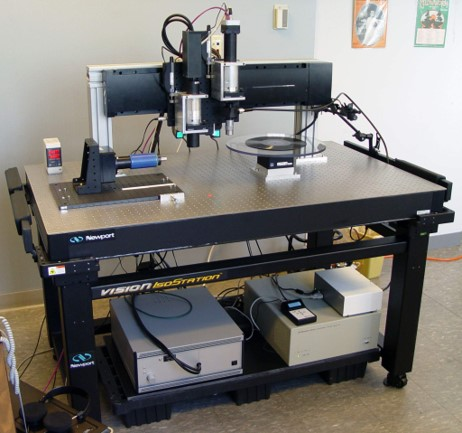
\includegraphics[width=0.5\textwidth]{../images/IRENE.jpg}
	\caption{IRENE (Source : lab's collection)}
	\label{irene}
\end{figure}

The 2D camera takes pictures of one line on the disc, 1 pixel high for 4096 pixels long. The pictures are taken at a very high frequency while the record is turning, imaging the disc line by line. The actual frequency is tuned for the support imaged.

To take pictures, light is directed with a certain angle on the disc. The sensors are activated by the reflected light, and write the perceived amount. Direct reflection results in white pixels, no light reflected becomes black, and in between are the gray scales.
\begin{figure}[H]
	\centering
	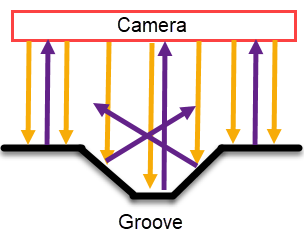
\includegraphics[width=0.5\textwidth]{../images/grooveside.png}
	\caption{Camera lighting the groove and detecting direct reflection (self-made diagram)}
	\label{grooveside}
\end{figure}
The grooves are usually made of large white bands outside (the disc surface), black bands inside (the groove's "walls"), and a thin white in the middle (bottom of the groove). Between these bands, there is a small area of gray scaled pixels.
\begin{figure}[H]
	\centering
	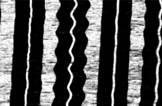
\includegraphics[width=0.5\textwidth]{../images/groove.png}
	\caption{Resulting image of grooves (source : LBNL collection)}
	\label{groove}
\end{figure}
Any kind of damage, texture, or unwanted object on the disc can be seen, as it disturbs light reflection. It is considered as noise on the image, and the reason the ML4NR project exists.
\subsection{Weaver}
Along with the IRENE system exists a program named Weaver, made in C\#. It is a collection of plugins developed through the years by researchers and students, used to pipeline the data reading process. 

Weaver's main function is to generate the sound wave from the imaged grooves, using an edge detection algorithm to find the exact center of the groove (figure \ref{edges}). However, since the images are noisy (dust, damage, texture), the sound generated also contains a high frequency background noise. Simply cutting the high frequencies wouldn't completely work, as the noise in images can also influence lower frequencies.

\begin{figure}[H]
	\centering
	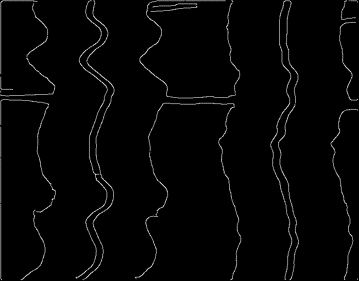
\includegraphics[width=0.5\textwidth]{../images/edges.png}
	\caption{Detected edges. Averaging them gives the center of the groove. (Source : LBNL collection)}
	\label{edges}
\end{figure}
\subsection{Machine learning and deep neural networks}
Machine learning is a powerful computing technique used for handling problems having too many parameters for a deterministic algorithm, for example object detection and classification in pictures, or market predictions. It is based on the ability to learn from given correct solutions in order to predict results of future inputs.

Deep neural network is a type of model inspired by the human brain. It is based on multiple layers of neurons. Each neuron takes some data as input, does some transformation, and feeds the output to the next neuron layer. By setting a goal (ground-truth), it can evaluate its result using a loss function, and change slightly the transformations occurring in all layers (weight adjustment). It repeats this process over and over until a threshold is passed.
\subsection{Shellac disc images properties}
This project is aimed at shellac discs, detailed in section \texttt{Mechanical Audio Records}. The LBNL has already imaged a lot of them, and so possesses a consequent collection of groove images.

The shellac discs were imaged at 104 KHz by IRENE, resulting in exactly 80,000 pixels for one revolution. However, those revolutions are divided in 8 parts of 10,000 pixels each. 

IRENE's 2D camera horizontal resolution is 4096 pixels. To obtain a good image quality, it was calibrated to take 3 microns per pixel. This means between 9 and 11 grooves are taken at the same time, and 15 to 30 revolutions are needed to image the entire disc.

So, each shellac disc is imaged with 8 x (15 to 30) pictures of 10,000 x 4096 pixels. All these pictures are in bitmap format and in gray scale.

\begin{figure}
	\centering
	\includegraphics[width=0.4\textwidth]{../images/Vaya-52212c.png}
	\caption{One image of the shellac disc of Vaya Con Dios, by Les Paul and Mary Ford (source : LBNL collection)}
	\label{vaya}
\end{figure}
\subsection{Audio data}
For some of the shellac discs, the LBNL possesses the audio source used to press them, coming from a tape. This gives us a clear reference on what the play back should sounds like. They were typically recorded at 44'100 Hz.

For the other discs, the audio reconstructed by Weaver can still serve as a good goal for the machine learning model. 

\section{Objectives}
The main goal of the ML4NR project is to generate a cleaner sound than the deterministic algorithm when given noisy groove images as input by using machine learning. It was never attempted before at the LBNL. The project is divided into progressive steps, each corresponding to a working prototype.
\subsection{Prototype 0}
This prototype serves as auto-formation for using KERAS. It'll teach the basics of model building. Its goal is to have a result on the CIFAR-10 dataset (not necessarily good). 
\subsection{Prototype 1}
This prototype is a proof of concept. Using Weaver, groove images of pure sine waves are generated. They are used to train a model, whose goal will be to find the simple frequency sound wave from the image. A metric needs to be defined for result evaluation.
\subsection{Weaver Plugin}
The previously used Weaver plugin needs to be modified, in order for it to be able to generate noisy groove images. The artificial noise needs to have the same properties as the real one from imaged grooves.
\subsection{Prototype 2}
This prototype tests the robustness of the model built before. It uses the noisy groove images generated with the Weaver plugin as input, and tries to find the clear sound wave. State of the art (SOTA) analysis helps improve the model.
\subsection{Prototype 3}
This prototype checks if complex sound waves can be generated by the model. Actual images of discs are used as input, and the goal is to find the same sound that is generated using the deterministic algorithm. Maybe a "bad result" regarding the goal could be better than current results.
\subsection{Prototype 4}
Final prototype, it uses the actual images of the discs, and the corresponding clean sound as goal. The clean sound is either obtained from a recorded stylus play, of from the original audio tape (which was used to print the disc). The results of this prototype are the results of the project.

If possible, this prototype is implemented as a plugin in Weaver.  
\section{Tasks}
\subsection{Prototype 0}
\begin{description}
	%	\item[n] d
	\item[Familiarize with KERAS and TensorFlow] Read documentation and set up a working environment for KERAS. Learn how to use.
	 \item[Analyze layer types] Read about the types of layer commonly used when building a machine learning model. Find specific ones for this context.
	 \item[Build own model] Create a model that can deal with pattern recognition, for handwritten characters.
	 \item[Train and test on MNIST dataset] Train model on MNIST dataset (handwritten numbers) and test accuracy/precision. No need to have good results, it is a proof of concept.
\end{description}
\subsection{Prototype 1}
\begin{description}
	%	\item[n] d
	\item[Analyze SOTA of sound generation] Analyze the current State of the Art in sound generation using machine learning.
	\item[Define a metric for model evaluation] Define which metric should be used to determine if a model is good or not.
	\item[Documentation of SOTA] Produce a written document on current SOTA, for future use.
	\item[Familiarize with Weaver] Learn how to use Weaver, the pipelining tool for IRENE.
	\item[Generate dataset of sine grooves] Use Weaver to generate a dataset of groove images whose base is a simple sine wave (one single frequency). The groove should be clean.
	\item[Create or use model for sound generation from images] Based on the SOTA, create or use a model able to generate sound from groove images.
	\item[Train and test model] Train the model with the dataset previously generated.  Use pure single frequency sound as ground-truth. Test with metric defined earlier. Improve the model and parameters to have better results.
	\item[Documentation of prototype] Document everything about the prototype.
\end{description}
\subsection{Weaver Plugin}
\begin{description}
	%	\item[n] d
	\item[Familiarize with plugin code] Read and understand the code of the Weaver groove image generator plugin.
	\item[Analyze structure and properties of noise] Analyze all the properties of actual discs images noise.
	\item[Implement modified plugin to generate noisy grooves] Modify the plugin so it can generate noisy grooves, with a noise having the same properties as actual discs images.
	\item[Document new plugin] Document everything used for this plugin, as well as noise properties.
\end{description}
\subsection{Prototype 2}
\begin{description}
	%	\item[n] d
	\item[Generate dataset of noisy sine grooves] Use previously implemented plugin to generate a dataset of images with grooves of simple sine waves, but noisy.
	\item[Train and test previous model] Try to train previous model with noisy images, and see what it can do. Use pure single frequency sound as ground-truth (not noisy sound). Use the metrics defined.
	\item[Analyze SOTA and leads to improve model] Use SOTA documentation and leads from workshops to improve the model and the results, regarding the metrics.
	\item[Document prototype] Document everything about the prototype.
\end{description}
\subsection{Prototype 3}
\begin{description}
	%	\item[n] d
	\item[Obtain dataset of imaged discs and generated sound] Obtain dataset of actual noisy grooves, imaged by IRENE, and their corresponding sound generated with Weaver.
	\item[Train and test previous model] Use model made for simple frequencies and test results. See if it can find the actual sound. The ground-truth is the noisy sound generated by Weaver.
	\item[Improve model with leads and SOTA] Check documentation and leads, improve model and parameters until it obtains a good result regarding the metrics.
	\item[Document prototype] Document everything about the prototype.
\end{description}
\subsection{Prototype 4}
\begin{description}
%	\item[n] d
    \item[Obtain dataset of imaged discs and recorded sound] Obtain dataset of actual noisy grooves, imaged by IRENE, and their corresponding sound recorded when played with a stylus. The sound could also come from the original tape.
    \item[Train and test previous model] Use model made previously and test results. See if it can find the actual sound. The ground-truth is the clean sound obtained by stylus play or from the original tape.
    \item[Improve as much as possible] Check documentation and leads, improve model and parameters until it obtains a good result regarding the metrics.
    \item[Document prototype] Document everything about the prototype.
\end{description}
\subsection{Integration to Weaver}
\begin{description}
	%	\item[n] d
	\item[Adapt code, I/O, to integrate with Weaver] If necessary, find a way to implement the model in a Weaver plugin, so it can be used for pipelining.
	\item[Document how to use] Document the plugin code and its usage.
\end{description}
\subsection{Planning}
See end of document. The PDF version is in high quality and can be zoomed on.
\subsection{Risks}
If the sound generation form images doesn't give good results, the method can be changed. A possible method would be to "denoise" the discs images or the reconstructed sound wave, using denoiser models of machine learning.

\section{Prototype 0}
This prototype's goal is to familiarize ourselves with Keras and TensorFlow, by implementing a simple model.
\subsection{Keras and TensorFlow}
TensorFlow is a Python and C API developed for machine learning\cite{tf}. It facilitates computation using flow graphs, and can be used on a GPU. Interconnected neuron layers are a flow graph.

Keras is a high-level API that can use TensorFlow as a basis for machine learning and neural networks\cite{keras}. It makes it easier for developers to implement deep neural networks (DNN) by having layer types already ready to use and ways to organize them. It also offers a lot of data manipulation for pre- and post-processing.
\subsection{CIFAR-10}
CIFAR-10 is a public dataset widely used for machine learning training and evaluation\cite{cifar}. It consists of 60,000 color images belonging to 10 classes (animals and vehicles). The goal is to be able to find the right class for a given image.
\begin{figure}
	\centering
	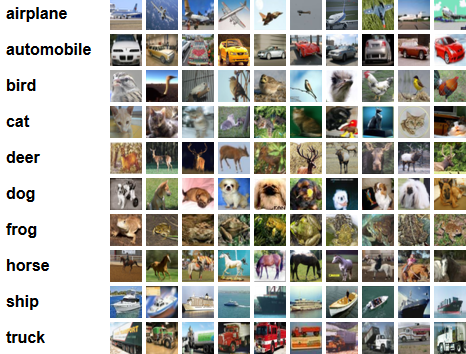
\includegraphics[width=0.8\textwidth]{../images/cifar.png}
	\caption{Example of images in the CIFAR-10 Dataset (source : \cite{cifar})}
	\label{cifar}
\end{figure}
\subsection{Convolutional Neural Networks}
Following the tutorials proposed on Keras website\cite{keras}, it seems convolutional neural networks (CNN) are a good way to start for image classification.

It is based on the principle of scaling: some features are small and very specific, while other are big and generic. CNN uses convolution to reduce the image's dimension while taking every pixel into account. The weights give more or less importance to some scales and positions in the picture. 

Putting multiple layers of convolutions completely interconnected let the model finds high-level information on the picture. Usually, in between layers there is an activation function, whose task is to put values in a certain range. 

Multiple iterations of 3-4 convolution layers + activation layers, followed by a max pooling layer, and ending with some fully connected layers, is the suggested way for image classification in their tutorial.
\subsection{Implementation and results}
The model is constructed as follow : 
\begin{figure}
	\centering
	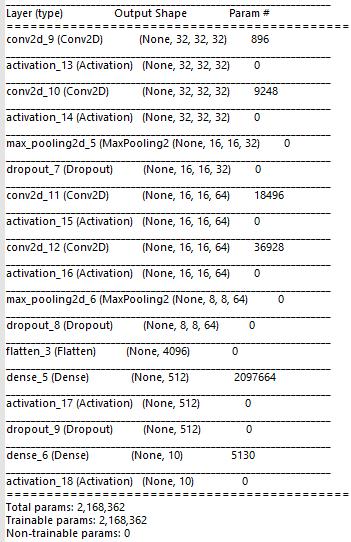
\includegraphics[width=0.8\textwidth]{../images/prototype0_summary.png}
	\caption{Architecture of the model for prototype 0}
	\label{prototype0_summary}
\end{figure}

It obtains around 75\% of accuracy for classification after only a few epochs
\section{Prototype 1}
This prototype will determine if it's possible to generate sound from an image. Its goal is to find the sound wave of a simple sine groove.
\subsection{SOTA machine learning models}
Over the years, multiple types of layers and neural networks were invented, each for a specific task\cite{aiml}. In this project, the goal is to generate precisely a sound wave from a groove image. It needs to be able to find the sound amplitude at a certain point on the groove. The amplitude is given by the perpendicular velocity of the needle when following the groove, meaning it's not the absolute position that is important, but the change of horizontal position.

Machine learning models generally try to find a solution for two types of problems : classification and regression.

Classification can be done while knowing what classes are possible, or just trying to cluster inputs together. If used with images, they are usually small (28x28 to 128x128).

Regression is the search of a continuous value. If the data points are time dependent, a typical problem is to predict the next value.

For classification, our problem (finding the amplitude at a given moment) could be seen as classifying small groups of groove lines into an amplitude, since they are discrete (encoded in 32 bits maximum, ~4 billions classes). This seems completely unreasonable.

For regression, the groove and sound could be seen as time series, and the goal would be to predict amplitude values.

Also, the problem can be seen as an interpolation one : given clean needle positions, what is the best curve to connect them ? Once determined, taking the derivative would give the sound wave.

If it is not possible to generate sound from images, other approaches can be taken (see Risks)

Here is a list of models, their application, and their relevance to our problem:
\begin{description}
	\item[Convolutional Neural Network - CNN] Can find detailed and general information on a picture, used for classification. Outputs a vector of class probabilities. This can be used for ML4NR by treating the output vector as a list of amplitudes in playing order.
	\item[Auto-encoder] Can remove noise by first finding the feature of the data while reducing it (encoding), and then expanding the feature to recreate the data (decoding). Used for image denoising, and interpolation. It can be used for this project.
	\item[Generative Adversarial Network - GAN] Composed of two parts competing against each other : one part tries to generate realistic data while the other tries to detect real and generated data. Used for dataset generation when real data is hard to obtain. Can be used for denoising. May apply in this project.
	\item[Residual Network - ResNet] Very deep network of convolutional layers (up to 150). The idea is to connect the input of a layer to the next layer, so they can learn by seeing processed and unprocessed data. Used for classification. Can be used here.
	\item[Recurrent Neural Network - RNN] Simple neural network, but the output of a layer is fed back to a previous layer. This allows it to learn from past values, and is good for time series. Used for regression. Can be used here.
	\item[Long Short-Term Memory - LSTM] Same idea as recurrent neural networks, it uses previous feature values to find the present output. The difference is the possibility to have as many previous data as needed. A special neuron is responsible for telling when a previous feature value is still relevant or not. Very good for time series, can be applied here.   
\end{description}
By tweaking the problem, all those models could be used. It is complicated to see what would be best, as no similar project were found. For this prototype, the first try is with a CNN model, like the one used in prototype 0. The second try is with a LSTM model.

\subsection{Risks}
If the model is really bad at finding the correct sound from the image, other methods could be used :
\begin{itemize}
\item Cleaning the image of its noise with an auto-encoder.
\item Finding the needle positions at successive time steps, and using the derivative to obtain the amplitude
\item Cleaning the generated audio of its noise
\end{itemize}

\subsection{Weaver plugins}
Weaver consists of more than 150 plugins, each doing a specific process. They are divided into categories : Load, Image, Track, Process, Save, Other.

All plugins inherit from the AbstractPlugin class, containing data useful to most of plugins. They are chained automatically when placed in the pipeline. 
\subsection{Dataset generation plugin}
A machine learning dataset needs to be as diverse as possible, in order to avoid over-fitting. A plugin able to generate a random dataset would be ideal.

A single Weaver plugin, named Create2D\_Sine, manages the generation of clean simple groove images. Different parameters can be chosen. A new plugin inspired by Create2D\_Sine is implemented in order to generate an entire dataset in one go, with the following ideas in mind:
\begin{itemize}
	\item The images should be random in an acceptable range.
	\item It should be possible to generate systematically all combinations if desired.
	\item The dataset size can become quite big, an estimation of the size would be useful.
\end{itemize}

All sine groove parameters can be randomized. The most intuitive way to do it is to take minimum, maximum and step for each parameter. Setting minimum = maximum will generate only this value for this parameter.

Figure \ref{dsplugin} shows the interface of the newly developed plugin.

\begin{figure}
	\centering
	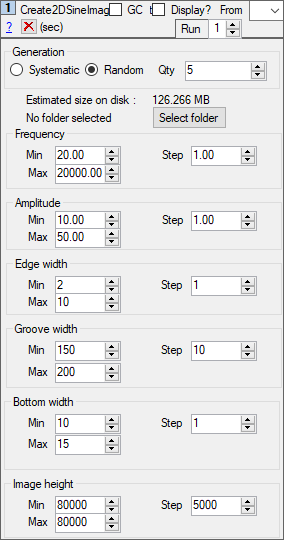
\includegraphics[width=0.5\textwidth]{../images/datasetplugin.png}
	\caption{Dataset generation plugin interface}
	\label{dsplugin}
\end{figure}

The generated groove file name contains the values used for each parameter. Then are encoded as the parameter's first letter and the value. Ex : f1875\_a10\_e3\_b12\_g160\_h80000.tif is a groove of frequency 1875 Hz, amplitude 10, edge width 3, bottom width 12, groove width 160, and 80'000 pixels of height.

Using Weaver loop plugin, the corresponding sound of each image is generated.
\subsection{Dataset}
Figure \ref{gengroove} shows what a generated groove looks like.
\begin{figure}
	\centering
	
\includegraphics[width=0.5\textwidth]{../images/example_groove.png}
	\caption{Generated groove, frequency=2760}
	\label{gengroove}
\end{figure}
The first idea is to generate randomized grooves so model inputs are as diverse as possible. However, the audio file generated from a random groove can sometimes be wrong. The algorithm used by Weaver plugins needs initial values close to the actual ones, and it's quite complicated with a random dataset. Furthermore, even the "correct" audio files contain some high frequency noise, due to the algorithm imperfection. We decide to generate the audio data from the code and not Weaver for this prototype.

The groove and image properties are fixed, for an easier manipulation of data for training. Only the frequency is randomized.
\begin{table}
	\begin{tabular}{|r|l|lll}
		\cline{1-2}
		Width        & 204        &  &  &  \\ \cline{1-2}
		Height       & 80'000     &  &  &  \\ \cline{1-2}
		Frequency    & 20 - 5'000 &  &  &  \\ \cline{1-2}
		Amplitude    & 10         &  &  &  \\ \cline{1-2}
		Edge width   & 3          &  &  &  \\ \cline{1-2}
		Groove width & 160        &  &  &  \\ \cline{1-2}
		Bottom width & 12         &  &  &  \\ \cline{1-2}
	\end{tabular}
\end{table}

In order to keep some space, we generate around 100 images.

So ideally, the input is a 204 x 80'000 8-bits image, and the output is a 104KHz 16-bits/channel stereo wave file.
\subsection{Model implementation}
\subsubsection{Version 1}
The first intuition is to use what we already know from prototype 0: the CNN layer.

The input is a 80'000 by 204 8-bits gray-scale groove image, and the goal is to find the WAV data of 80'000 samplings.
The audio file has two channels, even if most of the time they have the same value. Each channel is encoded in 16-bits. We only search for one channel and copy it for the second.

The first layer has to accept one groove image as input, as they are too heavy to all be loaded in memory. For each epoch, we loop through all images, feeding them one at a time to the model for fitting. The model is saved every epoch, because Google Colab, used for the implementations of this project, makes sessions expire after a fixed time.

\begin{figure}
	\centering
	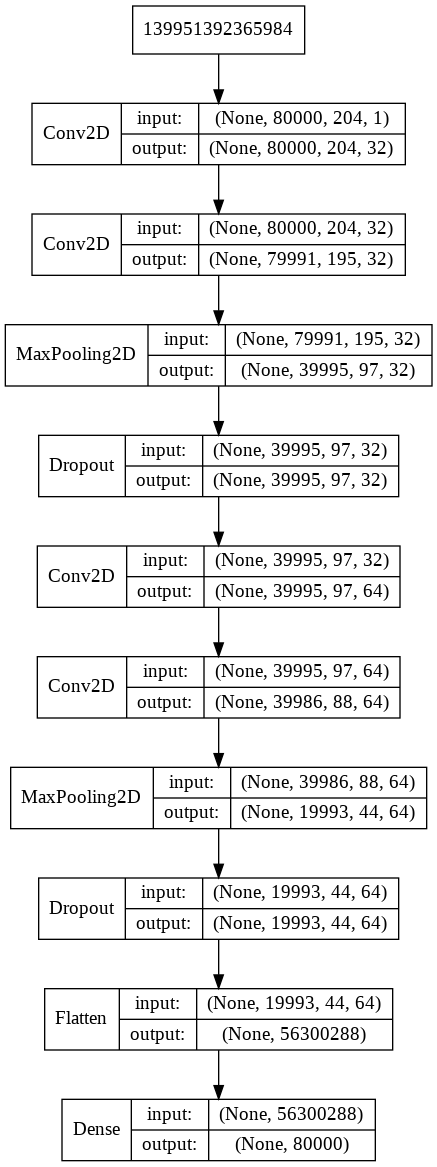
\includegraphics[width=0.5\textwidth]{../images/model_v1.png}
	\caption{Architecture of the convolutional network}
	\label{archiv1}
\end{figure}

\begin{figure}
	\centering
	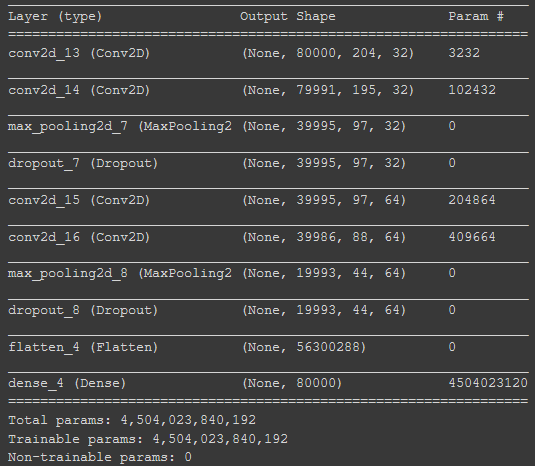
\includegraphics[width=0.7\textwidth]{../images/model_v1_params.png}
	\caption{Parameters count of the model}
	\label{paramv1}
\end{figure}

The convolutions kernel are 10x10 because 10 rows of data should help find the amplitude at a certain point, and 10 columns cover the groove edge. The output size of 32 is what is typically used in examples. Padding keeps the image at the same size.

A good optimizer is ADAM, who uses gradient descent. All parameters are left with default values. Mean square error (MSE) seems to be a perfect loss function for our problem, as the further we are from the ground-truth, the worse it is. Mean absolute error (MAE) can also provide insight on the results.

\subsubsection{Version 1 results}
After training for 10 epochs over 94 images, the best results are obtained by images whose audio contains a lot of 0. Their loss function score is however still horrible : in the order of 10'000s to 100'000s for MSE, 1000s for MAE. Images whose sounds have a lot of non-zero score in the order of 10'000'000s for MSE, and 10'000s for MAE.

Seeing that the loss scores increases over time, we know there is a problem with our parameters and/or inputs. 

Since it is a first shot at this problem through intuition, we decided to abandon this method and to search a better model.
\subsubsection{Version 2}
The first version being unsuccessful, we searched further in the current SOTA for regression problem linked to time series. A neural network that stood out was Long Short-Term Memory (LSTM)\cite{lstm}.

LSTM are composed of neurons able to retain information from previous steps. They use them to predict values, but if an input from a previous step is no longer useful, it's able to forget it.

In order to use it with Keras, the inputs needs to be reshaped in three dimensions. The first is blocks of multiple rows. The second is the rows of features for one prediction, also called time steps. The third is the features.


Since it already is a full Neural Network (it generates a node for each feature at each time step), we decided to use only one of them for now. It will take one block of rows as input at a time, and output the amplitude for both channel at that time step.

\begin{figure}
	\centering
	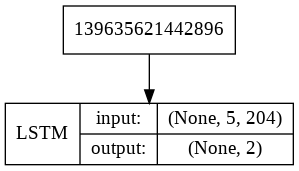
\includegraphics[width=0.5\textwidth]{../images/model_v2.png}
	\caption{Architecture of the LSTM network}
	\label{archiv2}
\end{figure}

\begin{figure}
	\centering
	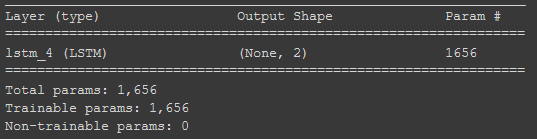
\includegraphics[width=0.7\textwidth]{../images/model_v2_params.png}
	\caption{Parameters count of the model}
	\label{paramv2}
\end{figure}

This model takes a 5 x 204 image as input, and gives 1 x 2 as output (the amplitude for both channels).

For the loss function and optimizer, we will keep the same as version 1.

\subsubsection{Version 2 - results}
After training for 10 epochs over 94 images, the results are in the same range as version 1. It seems the problem comes from the learning rate and the features, rather than the model itself.

\subsubsection{Version 3}
With version 2 results, we now know that the features are bad when used directly.

Following the advice of Mr. Hennebert, we normalize the inputs and target to obtain a nicer range. Each pixel of the groove image is normalized between 0 and 1. Each audio amplitude goal is normalized between -1 and 1.

Furthermore we use the CNN again, as it is easier to understand and fine tune. However, the input will have the same shape as in version 2 : a few rows of all pixels as input, and the amplitude of as output. Since the sound should be in mono, only one output value is needed.

\begin{figure}
	\centering
	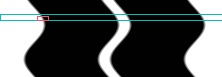
\includegraphics[width=0.8\textwidth]{../images/input.jpg}
	\caption{Window used to predict the amplitude}
	\label{input_v3}
\end{figure}

The blue rectangle is an example of input given to the model. The red rectangle is an example of convolutional kernel.

\begin{figure}
	\centering
	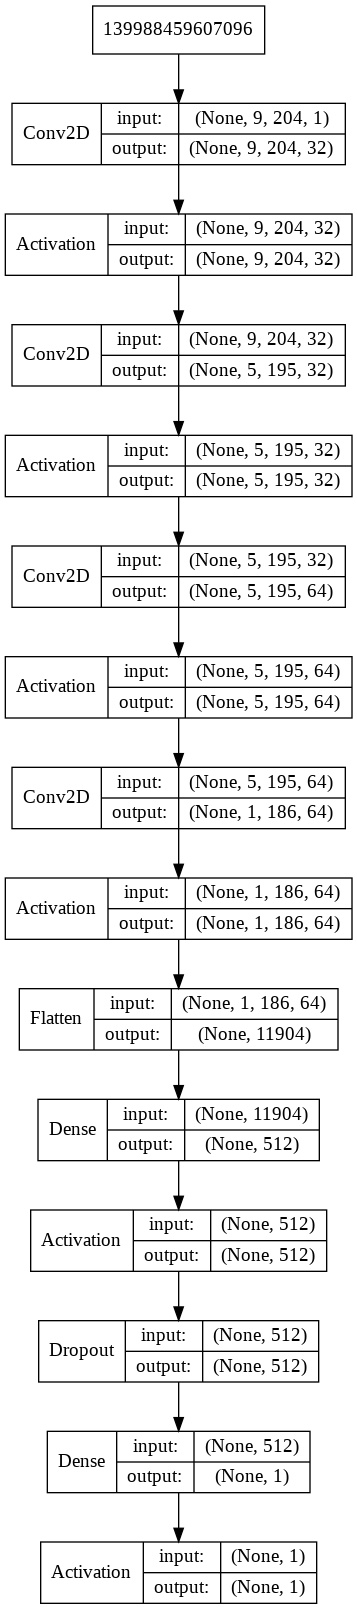
\includegraphics[width=0.3\textwidth]{../images/model_v3.png}
	\caption{Architecture of the CNN with window}
	\label{archiv3}
\end{figure}

\begin{figure}
	\centering
	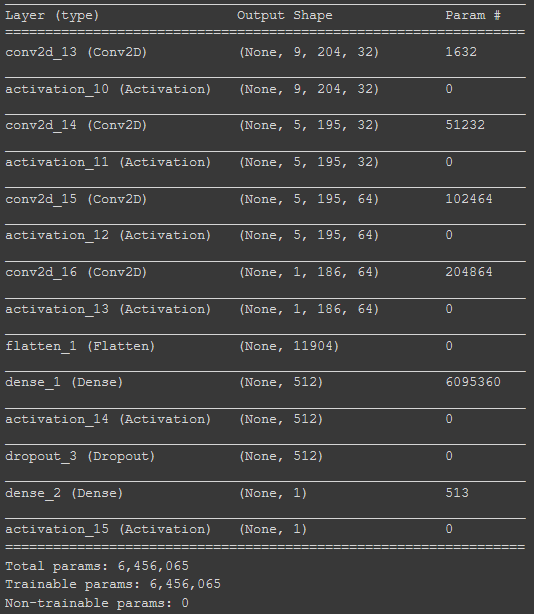
\includegraphics[width=0.7\textwidth]{../images/model_v3_params.png}
	\caption{Parameters count of the model}
	\label{paramv3}
\end{figure}

Each image is split into overlapping blocks of 9 rows and 204 features. They are then fed to the model, in which each convolutional layer tries to find hidden features in 5x10 matrices. 

For the two previous versions there were no activation layer, because the output wasn't bound. Here, since we are searching for an amplitude between -1 and 1, the tanh activation function seems reasonable.

The dropout layers make it harder to overfit.

The optimizer is also different : we use RMSprop, whose key advantage is the automatic adaptation of its learning rate. This avoids loss function triggering long jumps and divergence. The parameters used are learning\_rate=1e-4, decay=1e-6.

For validation, 15\% of the blocks of one image are taken out of training, and then used for scoring. Furthermore, after 25 images, a real sound generation is made from unseen images and saved (no scoring). This allows us to hear the results rather than comparing numbers.

\subsubsection{Version 3 - results}
This model seemed to have good results from the beginning, so everything was put in place to record the training : MSE and MAE scores for train and test images, weights saving, audio file registering.

Here are the MSE and MAE scores :

\begin{figure}
	\centering
	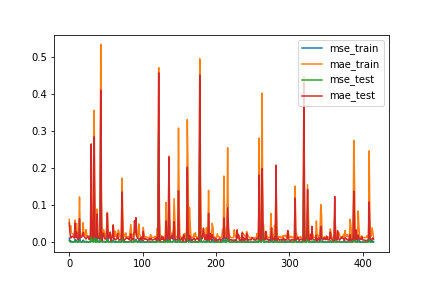
\includegraphics[width=0.8\textwidth]{../images/res_plot_v4.png}
	\caption{MSE and MAE for train and test scores}
	\label{scoresv3}
\end{figure}

We can see spikes. Those corresponds to low frequency grooves, where the lateral movement is really slow. We can see why the model has a hard time with them.

\begin{figure}
	\centering
	
\includegraphics[width=0.3\textwidth]{../images/low_freq.png}
	\caption{Groove of frequency 25}
	\label{lowfreq}
\end{figure}

A prediction of a low frequency groove has less amplitude, but the frequency itself seems to be correct.

\begin{figure}
	\centering
	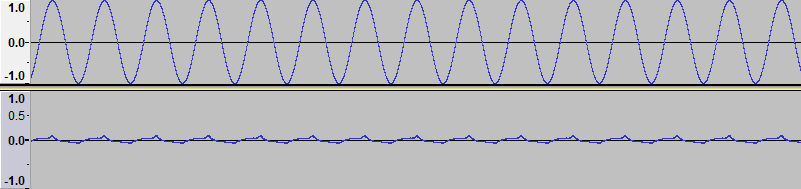
\includegraphics[width=1.0\textwidth]{../images/pred_60.png}
	\caption{Top : perfect sine wave of 60Hz / Bottom : predicted wave from groove}
	\label{pred60}
\end{figure}

Expanding the range after the generation could make it better.

As the frequency increases, the prediction is more spot on, and the audio sounds closer to the truth. 

\begin{figure}
	\centering
	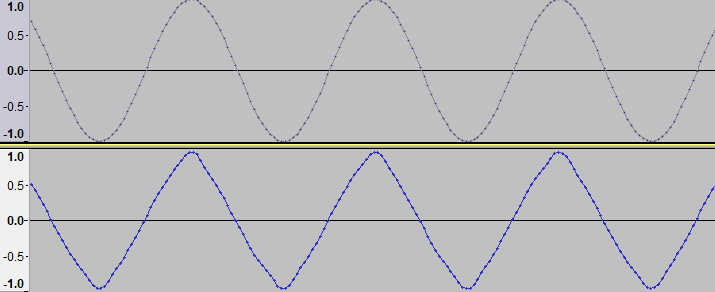
\includegraphics[width=1.0\textwidth]{../images/pred_2175.png}
	\caption{Top : perfect sine wave of 2175Hz / Bottom : predicted wave from groove}
	\label{pred2175}
\end{figure}

It is however very sharp, and analyzing the spectrum shows that a lot of higher frequencies are involved (mostly harmonics of our desired frequency).

\begin{figure}
	\centering
	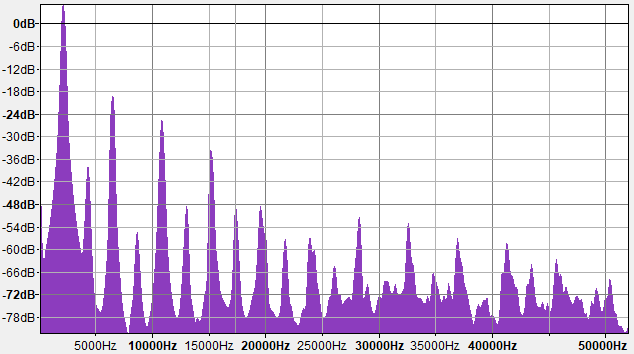
\includegraphics[width=0.8\textwidth]{../images/spectrometer_2175_v4.png}
	\caption{Spectrum of the generated audio for a 2175Hz groove}
	\label{spectrum2175}
\end{figure}

\subsubsection{Version 4}
In order to improve our results, fine-tuning all hyper-parameters is necessary. The success or failure of neural networks depends on it, as a bad combination could make the model and results diverge instead of converging.

The hyper-parameters of our model are :
\begin{description}
	\item[Batch size] Number of blocks given to train the network before updating the weights. Mainly depends on the memory available
	\item[Time steps] Number of rows of the sliding window. Too few and it will be hard to differentiate slopes of the groove. Too many and the model will take a long time to find what is useful.
	\item[Predictions] Number of amplitude points to find in one block. There may be a link between following amplitudes that the model can use to be more accurate.
	\item[Convolution filter shape] Convolution kernel size. Small filters can find smaller features, big ones can detect more general elements. Generally 3x3 in CNN.
	\item[Max pooling filter shape] Size of the kernel in which we keep only the maximum. Generally 2x2 in CNN.
	\item[Dropout rate] Proportion of neuron connections randomly cut to avoid over-fitting and accelerate learning time.
	\item[Activation function] Function that will collapse values on a certain range. \texttt{tanh} gives values between -1 and 1, \texttt{ReLu} between 0 and infinity.
	\item[Optimizer] Algorithm used to update the network weights. There exists a lot of them, with different properties and applications. Most of them need a learning rate and a decay rate.
	\item[Learning rate] Strength of the weight updates when searching the minimum loss. Too high and the values could diverge, too low and the learning will take a long time to find the minimum. 
	\item[Decay rate] Reduction of learning rate at every step, so it is less likely to diverge.
	\item[Loss function] Value calculated between predicted value and goal. This value is what the optimizer tries to minimize.
\end{description}

This makes a lot of parameters, and testing all possible combinations is impossible. Some of them seem to be more linked than others, and using intuition, are grouped like that :
\begin{enumerate}
	\item Time steps, predictions, and convolutional filter shape
	\item Max pooling shape and dropout
	\item Optimizer, learning rate, and decay rate
\end{enumerate}
Batch size can be fixed, as it should not have too much of an influence (32 is generally used). Loss function can also be fixed. For regression problem. a mean square error seems perfect.

Since the dataset is not noisy like the actual grooves, some of the parameters found here may not be ideal later. For this reason, the models are not trained for too long. One pass over all images should be enough to find the good combinations.

The input dataset is 78 images, each of them decomposed in up to 79'996 blocks using a sliding window. 15\% of them are taken away for validation, resulting in up to more than 5'300'000 blocks for training one epoch. The model trains on each block individually to find a certain number of predictions per block. This dataset should be big enough to have interesting results after one pass only.

In table \ref{hp1}, values considered for the first group of hyper-parameters can be found.
\begin{table}[H]
	\begin{tabular}{|r|l|l|l|l}
		\cline{1-4}
		Hyper-parameter				& Min	& Max 					& Step 	& \\ \cline{1-4}
		Time steps  				& 5    	& 9   					& 2    	& \\ \cline{1-4}
		Predictions 				& 1    	& Time steps  			& 2 	& \\ \cline{1-4}
		Convolution filter height  	& 3 	& Time steps / 2 + 0.5 	& 2 	& \\ \cline{1-4}
		Convolution filter width  	& 3 	& 9 					& 2 	& \\ \cline{1-4}
		
	\end{tabular}
	\caption{Range of values for hyper-parameters fine tuning}
	\label{hp1}
\end{table}

This already results in 104 possible combinations. In order not to lose too much time, only the 50 first combinations will be trained. If the best results are obtained with parameters values close to those that aren't trained yet, the remaining combinations will also be trained. However, if the best models are the ones with small parameter values, there is probably no need to train models with bigger values.

The other hyper-parameters seem more dependent on whether the dataset is noised or not, so they will be fine-tuned in prototype 2. 
\subsubsection{Version 4 results}
For result evaluation, every model tries to predict the audio wave of the 18 test images. The mean square errors of each prediction are averaged together to obtain the global test result.

The best results, after training over 78 images of grooves with variable frequency, are obtained by the first model tested (results of best three models in figure \ref{resp1v4}).

\begin{figure}
	\centering
	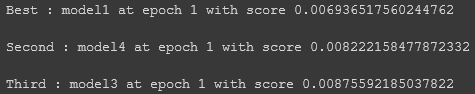
\includegraphics[width=0.8\textwidth]{../images/resp1v4.png}
	\caption{Top three results obtained by different combinations}
	\label{resp1v4}
\end{figure}

All three models have small hyper-parameters values : all have time steps = 5, predictions = 1, and convolution filter height = 3. The only difference between them is convolution filter width, which is in order 3, 7 and 9.

All the other results can be found in the appendices.

It can be assumed that there is no need to train models with bigger parameter values.

In table \ref{hpm1}, you can find the values used by the best model.

\begin{table}
	\begin{tabular}{|r|l|lll}
		\cline{1-2}
		Time steps        & 5        &  &  &  \\ \cline{1-2}
		Predictions       & 1     &  &  &  \\ \cline{1-2}
		Convolution filter    & 3x3 &  &  &  \\ \cline{1-2}
		Max pooling filter    & 2x2        &  &  &  \\ \cline{1-2}
		Dropout rate   & 0.25 (firsts) and 0.5 (last)          &  &  &  \\ \cline{1-2}
		Activation function & ReLu (firsts) and tanh (last)        &  &  &  \\ \cline{1-2}
		Optimizer & RMSprop         &  &  &  \\ \cline{1-2}
		Learning rate & 1e-4         &  &  &  \\ \cline{1-2}
		Decay rate & 1e-6         &  &  &  \\ \cline{1-2}
	\end{tabular}
	\caption{Hyper-parameters used for best results}
	\label{hpm1}
\end{table}

The model architecture can be found in the appendices.

For reference, the goal and predicted signals can be seen in figure \ref{predm1}.
\begin{figure}
	\centering
	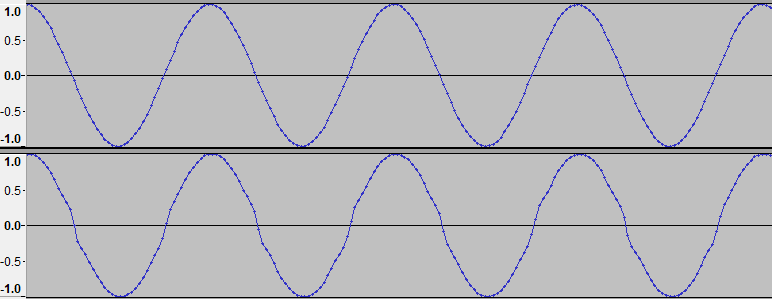
\includegraphics[width=0.8\textwidth]{../images/predm1.png}
	\caption{Top : goal signal of 2175Hz. Bottom : predicted signal}
	\label{predm1}
\end{figure}
Compared to the previous prediction of the same groove (figure \ref{pred2175}), this one looks better, especially at the peaks.

The spectrum (figure \ref{spectrumm1}) also shows a big difference between the main frequency and the overtones, indicating a reduced background noise
\begin{figure}
	\centering
	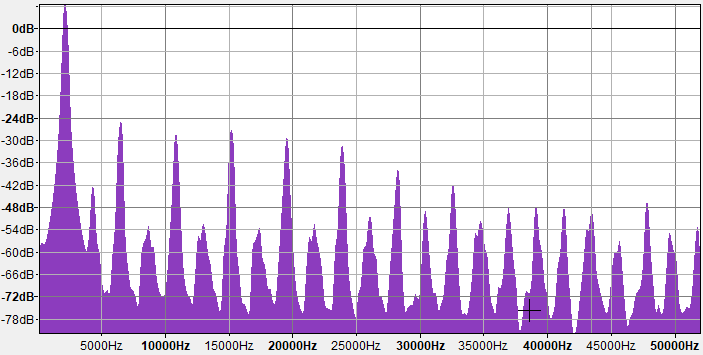
\includegraphics[width=0.8\textwidth]{../images/spectrum_m1.png}
	\caption{Spectrum of the predicted audio wave}
	\label{spectrumm1}
\end{figure}
\section{Prototype 2}
In this prototype, the goal is to train a model on noisy images of single frequency grooves and make it predict a perfect sine wave.
\subsection{Noisy groove images}
As can be seen in figure \ref{vayabis}, the actual disc images are noisy. 
\begin{figure}
	\centering
	\includegraphics[width=0.4\textwidth]{../images/Vaya-52212c.png}
	\caption{One image of the shellac disc of Vaya Con Dios, by Les Paul and Mary Ford (source : lab's collection)}
	\label{vayabis}
\end{figure}
That noise can be decomposed in different type of noise :
\begin{itemize}
	\item A light Gaussian noise that gets heavier on the groove edges, caused by dust and texture.
	\item Thin scratches that are seen as black.
	\item Bigger damage that is also seen as black.
\end{itemize}
All those makes the task of finding the sound more difficult, it is therefore important to simulate them for model training.
\subsection{Artificially noised dataset}
Since a dataset of grooves and their output is already available, a simple program can be used to noise them and generate a new dataset. Those noised grooves should look as much as possible as the actual disc images.

The Gaussian noise can be added easily on the perfect groove image. The black part should stay as dark as possible, and the white part should have visible deterioration. Knowing that the pixel values are between 0 and 255, a Gaussian noise of average -100 and standard deviation of 50 is clearly visible on the white parts and not so much on the black ones.

For the scratches, thin long black rectangles are generated randomly and placed randomly across the image.

For the big damage, the same is done with bigger black rectangles, but not as many as scratches.

The result of artificial noising can be seen in figure \ref{cleannoisy}.

\begin{figure}
	\centering
	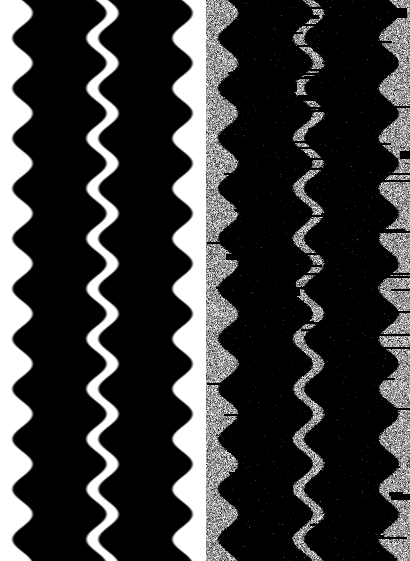
\includegraphics[width=0.5\textwidth]{../images/cleannoisy.png}
	\caption{Left : clean groove of 2075 Hz. Right : same groove artificially noised}
	\label{cleannoisy}
\end{figure}

\subsection{Version 1}
In this version, the dataset is the same as for prototype 1 (78 images for training, 18 for testing). All the images are noised once and written in static memory, so the training and testing images are the same for all models.

The goal is to obtain a good prediction of the sound wave of a noisy groove image. In order to do that, further fine tuning is necessary.
Instead of trying every combination like before, parameter values are tuned through trial and error.
\subsubsection{Implementation}
The first model trained is the one that obtained the best results in prototype 1.

Then, fine tuning over the learning and decay rate are tried. In the first model RMSprop is used, and the values are learning = 1e-4, decay = 1e-6. However, Keras documentation suggest using default values, which are learning = 1e-3 and decay = 0. We can also try to make the decay bigger to see how it affects learning.

Seeing the noised images, it seems a bigger sliding window could help find amplitude more easily when the groove edge is damaged. Big jumps in values make it faster to see if it's relevant or not to change it, so the network is tested with window height (time steps) of 5, 9, and 15.

Each model is trained over a varying number of epochs, depending on the occasional crash of the connection and the time taken.
\subsubsection{Results}
First come the results between the different learning and decay rates. Figure \ref{resp2v1lr} shows the results of the three best model and epoch.
\begin{figure}
	\centering
	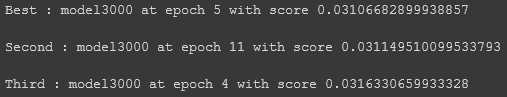
\includegraphics[width=0.8\textwidth]{../images/resp2v1lr.png}
	\caption{Top three results among all epochs and models where learning and decay rates are tuned}
	\label{resp2v1lr}
\end{figure}

The model using learning rate = 1e-4 and decay rate = 1e-6 obtains the three best results. However, the results don't seem to improve over time. It can be a sign of bad values or even bad optimizer. 

Next, using the default values of the RMSprop optimizer, the window height parameter is played with. Again, figure \ref{resp2v1ts} shows the results of the three best model and epoch.
\begin{figure}
	\centering
	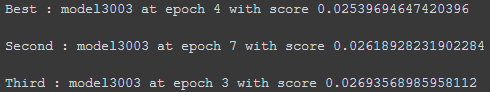
\includegraphics[width=0.8\textwidth]{../images/resp2v1ts.png}
	\caption{Top three results among all epochs and models where sliding window size is tuned}
	\label{resp2v1ts}
\end{figure}

This time, the results are a bit better. The best model is the one using a window height of 15 pixels. Our intuition proved to be right.
\subsection{Version 2}
In this version, a new dataset is used : groove images are now lightly randomized (groove width, edge width, bottom width), and they are noised on the fly during training. The test dataset is noised once, written in memory, and used for every model so comparisons make sense.

The training dataset contains 170 images, the test 30 images. 15\% of image blocks are used for validation. This makes training for one epoch quite long (around 3 hours with our current environment). Furthermore, a good result over the test set could be obtained in the middle of an epoch. With these two arguments in mind, a modification was made to th program : it is now possible to divide the training dataset and to test results after each smaller division. This also allows to resume training in case of crash.

In the previous version, the optimizer didn't seem to work correctly even with different values. In this version, other optimizers are tested : Adagrad and Adam.
\subsubsection{Implementation}
First, the best hyper-parameters previously found are used to train on the dynamic dataset. The same data is never seen twice, so the model should be more robust.

Then, optimizers Adagrad and Adam are tested with their default values.

The training dataset is divided in 10 smaller parts, and after each of them the model is tested.
\subsubsection{Results}
The model combining the best hyper-parameters and RMSprop optimizer trained over 6 epochs. The best results are obtained on epoch 1, showing that there is indeed a problem with the optimizer. However, it was used to make a prediction and see if the model can find the audio of a noised groove.

Figure \ref{groove1530} is the noisy groove used for test (never seen during training). Figure \ref{predm4000} is the perfect wave and the predicted one. Figure \ref{spectrum4000} is the spectrum of the predicted audio wave.
\begin{figure}
	\centering
	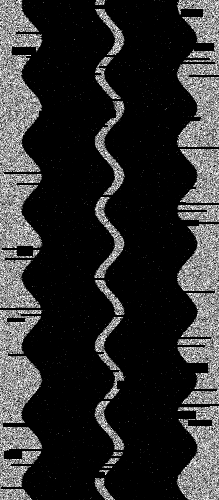
\includegraphics[width=0.4\textwidth]{../images/groove1530.png}
	\caption{Noisy 1530 Hz groove image used for testing}
	\label{groove1530}
\end{figure}
\begin{figure}
	\centering
	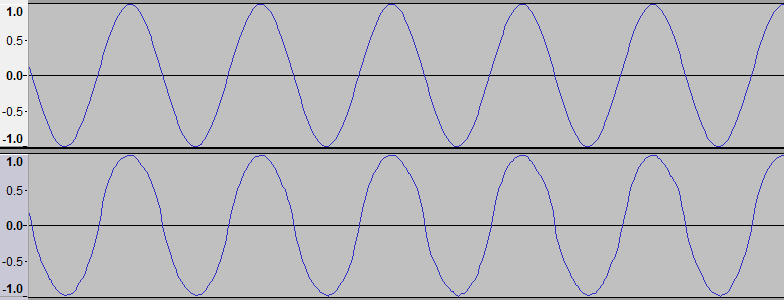
\includegraphics[width=0.8\textwidth]{../images/predm4000.png}
	\caption{Top : perfect 1530 Hz wave. Bottom : predicted wave from noisy groove image}
	\label{predm4000}
\end{figure}
\begin{figure}
	\centering
	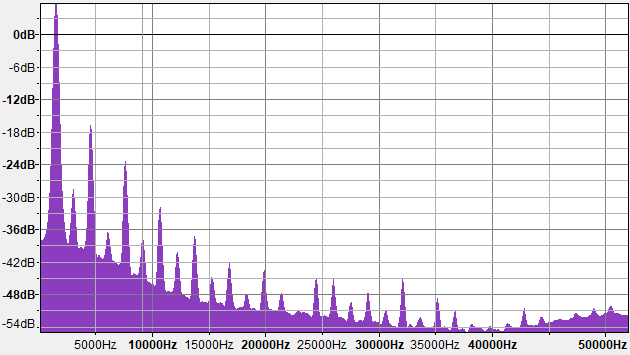
\includegraphics[width=0.8\textwidth]{../images/spectrum_m4000.png}
	\caption{Spectrum of the predicted 1530 Hz wave}
	\label{spectrum4000}
\end{figure}
The predicted wave looks thicker on the peaks. We can see that there are still overtones, however they quickly lose intensity. The predicted wave has some irregularities, but they are really small compared to the rest. It seems that even though it doesn't converge, this model is robust enough to predict a sound wave from a noisy image.

The next model to test has the same hyper-parameters except for the optimizer. It uses Adam with its default rates. The best test results are obtained at epoch 2.6. This epoch weights are used to make a prediction on the same groove as before. In figure \ref{predm4004} we can see the predicted sound wave on third position, the second being the prediction using RMSprop optimizer.
\begin{figure}
	\centering
	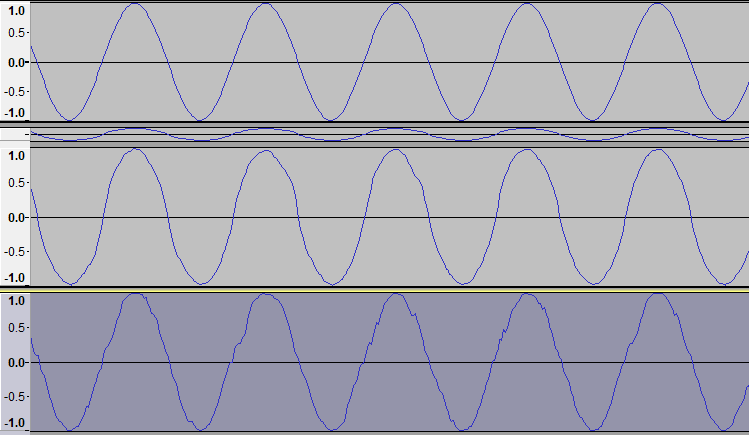
\includegraphics[width=0.8\textwidth]{../images/pred4004.png}
	\caption{Top : perfect 1530 Hz wave. Middle :  predicted wave from noisy groove image with RMSprop. Bottom : predicted wave from noisy groove image with Adam}
	\label{predm4004}
\end{figure}
We can see that the general shape is more similar to the perfect wave, however there are sharper errors. The spectrum (figure \ref{spectrum4004}) also shows overtones with less amplitude. It is a better result altogether.
\begin{figure}
	\centering
	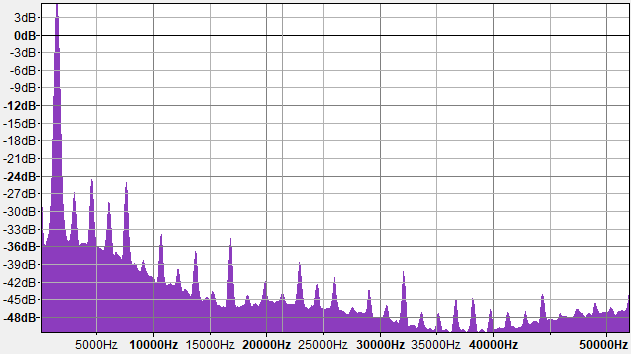
\includegraphics[width=0.8\textwidth]{../images/spectrum_m4004.png}
	\caption{Spectrum of the predicted audio wave}
	\label{spectrum4004}
\end{figure}
\section{Prototype 3 and 4}
The goal of this prototype is to obtain a clean sound wave from real disc images. There are three alternatives to try and find the audio from disc images :
\begin{itemize}
	\item Giving disc images directly to a previous model, and see what it can find.
	\item Continue the training of a previous model but with actual disc images as input and clean tape audio as goal (transfer learning).
	\item Train a new model only on disc images and tape audio.
\end{itemize}

Prototype 3 as described in the project objectives is abandoned. Indeed, training a model on noisy disc images with a noisy sound wave as goal seems it would only make it learn to include said noise in his predictions.
\subsection{Dataset}
Over the years, multiple discs have been imaged by researchers at the LBNL. Among those, 4 discs are available with their original tape audio. These seem perfect for the project, however they need some manipulation to be usable.

Each disc is digitized in multiple 80'000 by 4096 images. One image represents a complete revolution of the disc, but only covers around 10 grooves in width. 15 to 30 of those images are needed to represent the entire disc. Because the camera is placed and calibrated manually, the images overlap. Furthermore, each image is divided in 8 parts of 10'000 by 4096 pixels for storage. Those part don't overlap, and a Weaver plugin can merge them to obtain the bigger images.

For each of the 80'000 by 4096 images, multiple audio files have been generated using Weaver and its edge detection algorithm, trying different combinations.

The audio coming from the original tape is the audio of the entire disc. It is very clean, as no background noise can be heard. Figure \ref{spectrum_johnny} shows the spectrum of one of those tape audio : Johnny is the boy for me by Les Paul and Mary Ford. 

This audio is sampled at 44'100 Hz, but since IRENE has an imaging frequency of 104'000 Hz for shellac discs, it would be better to re-sample to also be at 104'000 Hz instead.

\begin{figure}
	\centering
	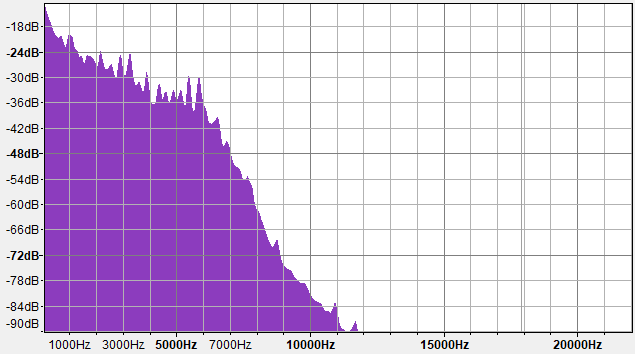
\includegraphics[width=0.8\textwidth]{../images/spectrum_johnny.png}
	\caption{Tape audio spectrum of Johnny is the boy for me by Les Paul and Mary Ford (generated in Audacity\cite{audacity} with Hanning window)}
	\label{spectrum_johnny}
\end{figure}

We need the disc images to match with the tape audio. There are two reasonable workarounds to do that :
\begin{itemize}
	\item Divide the tape audio in parts corresponding to each 80'000 by 4096 image.
	\item Merge all disc images, searching for overlapping parts.
\end{itemize}

It is worth noting that each 80'000 by 4096 image takes around 300 MB of space. This means that an entire imaged disc takes between 4.5 and 9 GB of space. While this is reasonable for non-volatile memory, that space is needed in RAM when actually merging the images, and our computer is not powerful enough for this. As so, the first workaround seems to be the best choice.

Since there are no indication on where the audio starts on the disc, we need to search manually for the right part. Weaver can help us for that : using the edge detection algorithm, the audio of one 80'000 by 4096 image is generated. Then, this audio is compared and aligned with the tape audio by eye and ear in an audio editing software (Audacity\cite{audacity} was used for this project). It can be seen in figure \ref{aligning}.

\begin{figure}
	\centering
	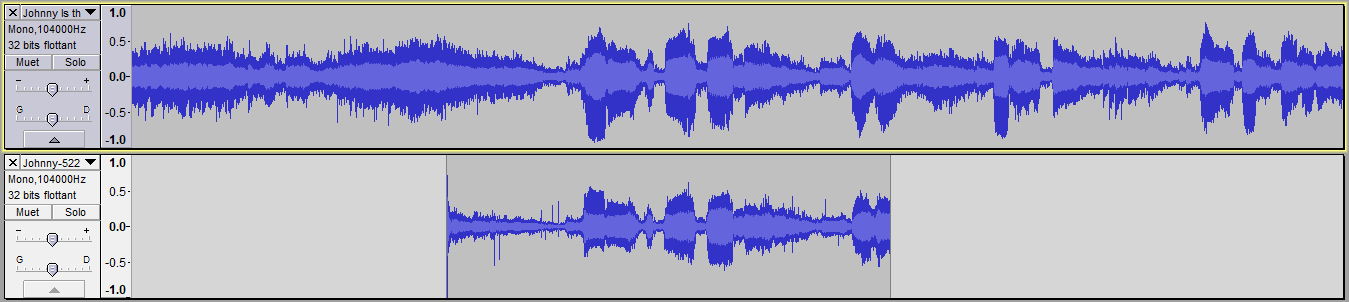
\includegraphics[width=1.0\textwidth]{../images/aligning.png}
	\caption{Trying to align the generated audio on the clean tape audio. Top : tape audio. Bottom : Weaver generated audio}
	\label{aligning}
\end{figure}

The rest of the tape audio is cut out. The clean audio corresponding to one image is now available.

The last problem comes from the images themselves. Since they cover multiple grooves (it is one groove, connecting at the top and bottom), we need a way to isolate them. It is not possible to divide the image in straight bands containing one groove each, because of a common defect in discs : the middle hole is not perfectly centered. It provokes a global shift in groove position. Figure \ref{moving_groove} is a vertically compressed 80'000 by 4096 image showing that shift.

\begin{figure}
	\centering
	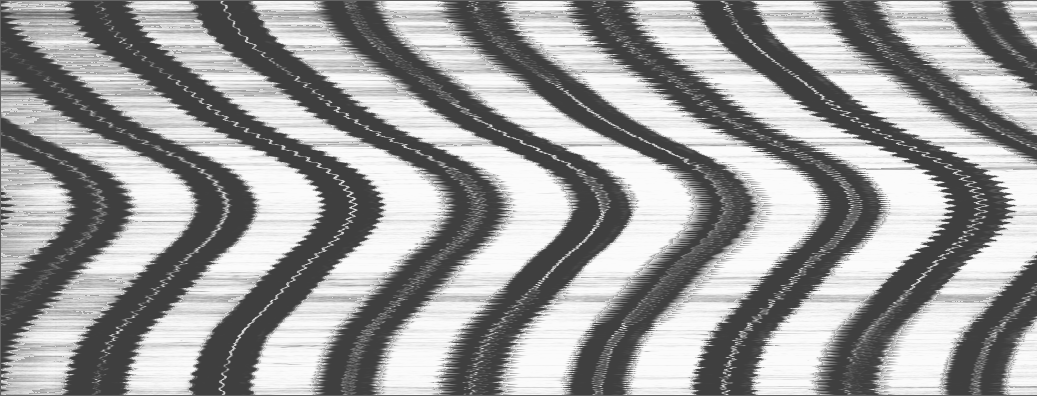
\includegraphics[width=1.0\textwidth]{../images/moving_groove.png}
	\caption{Vertically compressed 80'000 by 4096 image. A global '>' shape can be seen when following the grooves, provoked by a slightly off-center hole.}
	\label{moving_groove}
\end{figure}

Again, using Weaver's edge detection algorithm can help. It is used to find the middle of the grooves at each line and for each of them. It is imperfect because of the image's noise, but it is enough for what we want : each point of the newly found track is used as the center of a sliding window. In figure \ref{track_plugins}, the plugins used for edge detection and their parameters can be seen. Figure \ref{track_johnny} shows the track actually found.

\begin{figure}
	\centering
	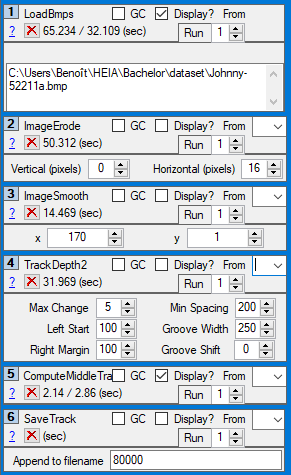
\includegraphics[width=0.4\textwidth]{../images/track_plugins.png}
	\caption{Chain of Weaver plugins and their parameters used for edge detection on disc images.}
	\label{track_plugins}
\end{figure}


\begin{figure}
	\centering
	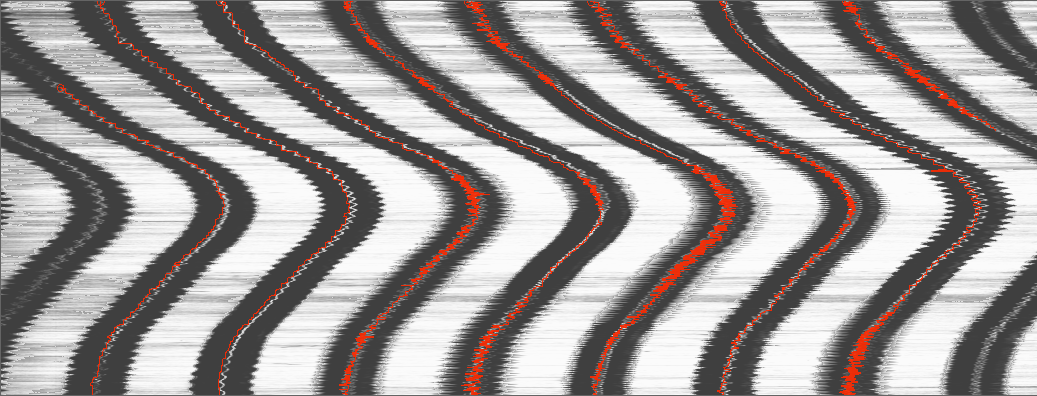
\includegraphics[width=1\textwidth]{../images/track_johnny.png}
	\caption{In red, track representing the middle of the grooves, found by Weaver.}
	\label{track_johnny}
\end{figure}

All parts are now ready for machine learning : groove image used for input, the track for the sliding window, and the clean audio goal, with one amplitude for each track position.

\subsection{Direct prediction}
First, let's see what happens when we try to predict the audio from the image using a model trained on simple noisy grooves.

The real disc groove is actually wider than the ones used until this point. The real grooves are around 240 pixels wide, and the previous models used grooves of 160 pixels. It means a new model has to be trained with the correct dimensions. More noise is also added on each image, to make the model more robust to noise. The complete list of Weaver generated grooves can be found in the appendices.

Following the same idea as prototype 2, the images used for training are noised on runtime and the ones used for testing are noised and stored before, so that tests can be compared (see figure \ref{noisy_proto4} for an example). The properties of each test image, the parameters of the noising function, and the seed used for randomization are given in the appendices.

\begin{figure}
	\centering
	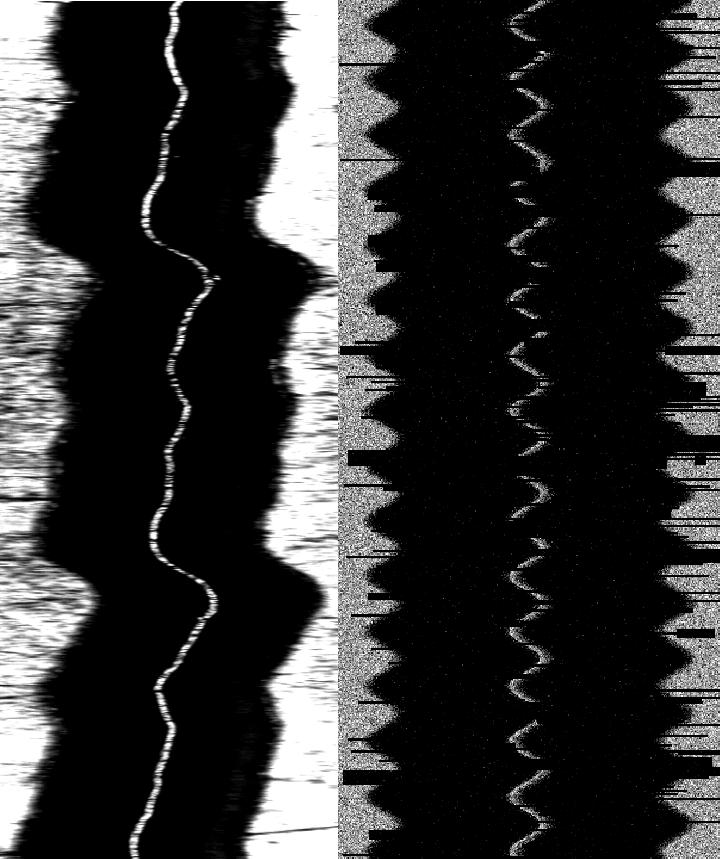
\includegraphics[width=0.6\textwidth]{../images/noisy_proto4.png}
	\caption{Right : Example of a noisy image used for testing. Left : Actual disc groove}
	\label{noisy_proto4}
\end{figure}

The model hyper-parameters are the one that obtained the best results in prototype 2, except for the sliding window width. It should cover all four edges of the groove. To compensate off-centered tracking points, it needs to be larger than the groove width : 320 pixels seems good. After training for a few epochs, results are compared (figure \ref{model_5000_res}) to select the best version.

\begin{figure}
	\centering
	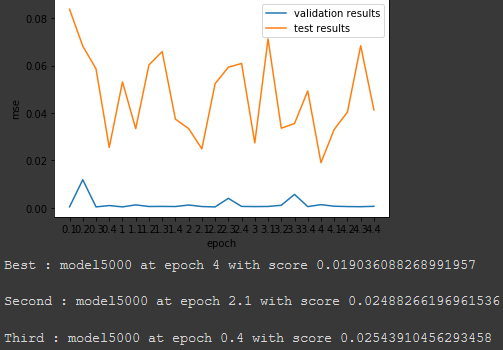
\includegraphics[width=0.8\textwidth]{../images/model_5000_res.png}
	\caption{Graph of the validation and test results obtained }
	\label{model_5000_res}
\end{figure}

Epoch 4 gives the best result over all test images, never seen during training. A prediction is made with this model on one of the test image. Figure \ref{comp_m5000} shows the predicted audio wave.

\begin{figure}
	\centering
	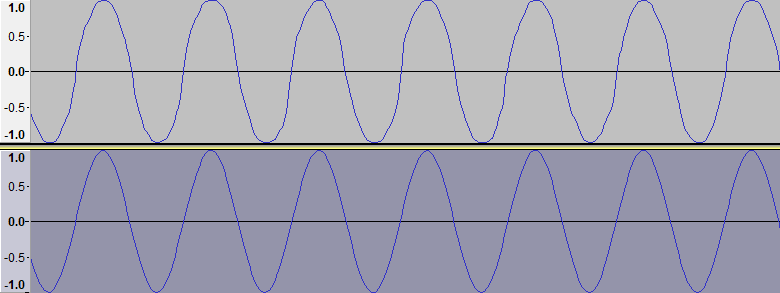
\includegraphics[width=0.8\textwidth]{../images/comp_m5000.png}
	\caption{Top : predicted audio wave of a noisy 1850 Hz groove. Bottom : perfect audio signal of 1850 Hz.}
	\label{comp_m5000}
\end{figure}

It looks like a good prediction.

Only one 80'000 by 4096 image will be used, as it represents around 5 seconds of audio data. It is consequent enough for what we are trying to obtain.

The chosen image is called Johnny-52211 in the LBNL database.

Using the disc groove track generated with Weaver, sliding windows are given to the model for prediction. For this image, there are more than 550'000 windows to predict from. Figure \ref{proto4_v1_wave} shows the audio wave predicted for the image compared to the actual audio from the tape.

\begin{figure}
	\centering
	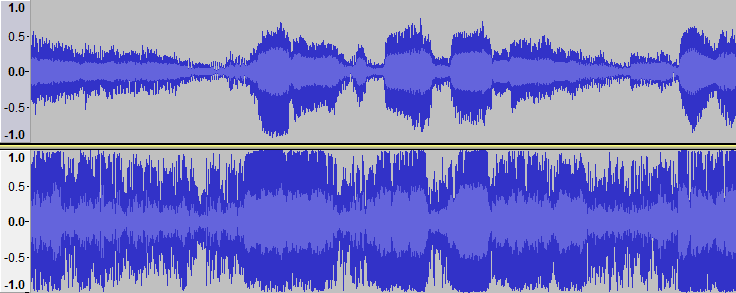
\includegraphics[width=0.8\textwidth]{../images/proto4_v1_wave.png}
	\caption{Top : Audio from tape. Bottom : Predicted audio using disc image}
	\label{proto4_v1_wave}
\end{figure}

We can already see that there is a lot of noise. The spectrums in figures \ref{spectrum_tape} and \ref{spectrum_m5000} show that the noise is spread on all frequencies.

\begin{figure}
	\centering
	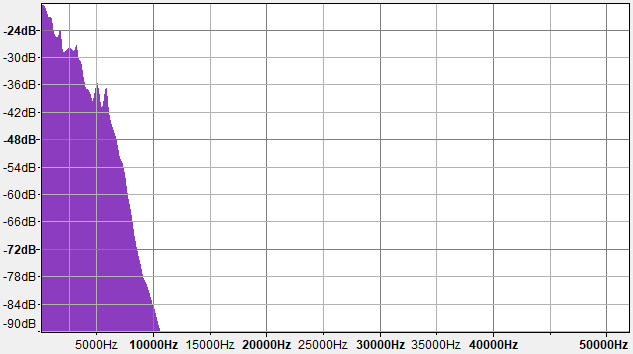
\includegraphics[width=0.8\textwidth]{../images/spectrum_tape.png}
	\caption{Spectrum of the tape audio corresponding to the Johnny-52211 image}
	\label{spectrum_tape}
\end{figure}

\begin{figure}
	\centering
	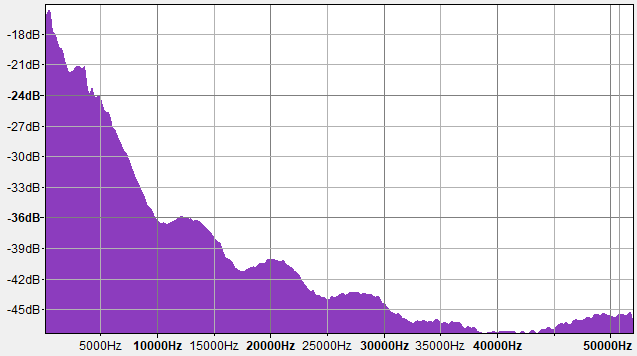
\includegraphics[width=0.8\textwidth]{../images/spectrum_m5000.png}
	\caption{Spectrum of the predicted audio wave on image Johnny-52211}
	\label{spectrum_m5000}
\end{figure}

Trying to directly make predictions in a model that has never seen disc images doesn't give good results. The next step is to train the model further using disc images.

\subsection{Transfer learning}
Transfer learning is a method used in machine learning for problems similar to other already known problems. For example if you need to classify animals into horse or lama, and you have a access to a model that was trained for cats and dogs classification, transfer learning can probably be used.

The main idea is to use the already trained weights as initial values for your model. If the input or output shape are different, the trained model can be wrapped by new layers to accept the new shapes.

In our case, the first model was made so that it would already take the right shape of input. The model can simply be loaded in the software and further trained with disc images.

The main problem comes from giving the goal to the model. The clean tape version of the sound wave is available, but there is no way to know exactly which point of the groove corresponds to which audio wave sample. As explained in the 8.1 Dataset section, one way to do it is to manually align the clean sound with a Weaver generated one. 

However, it is far from easy. The Weaver generated audio wave is imperfect : it has a bigger amplitude range, high frequency waves, and a different shape on most sections, making impossible to perfectly align. Our model takes a window of pixels as input, and one amplitude as goal : we need the amplitude to corresponds to one of the line in the window. Figure \ref{proto4_matching_detal} shows what the data looks like.

\begin{figure}
	\centering
	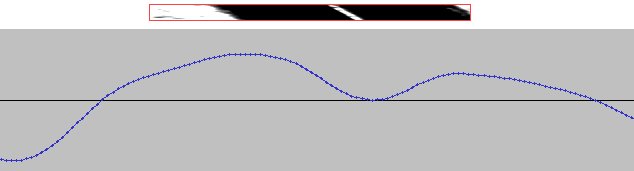
\includegraphics[width=1.0\textwidth]{../images/proto4_matching_detal.png}
	\caption{Inside the red rectangle : one window of pixels given to the model. Under : the audio wave from the tape. Only 15 of the audio data points match the window : which ones ?}
	\label{proto4_matching_detal}
\end{figure}

After manually aligning the Weaver generated audio to the tape audio as best as possible, the tape audio is cut to have the same amount of data points as the track of the groove. Since it is not sure that everything is matching correctly, only one image is used to train the model. We at least want good results on validation data (15\% of the windows are not given to the model for training and are used after to evaluate it).
Since there is a lot of windows (more than 550'000), the model is trained little by little to avoid running out of RAM. Only 50'000 windows are loaded at a time.

After training on the entire image 10 times, a sound prediction of the same image is made. Audio wave can be seen in figure \ref{m5001_pred}, and its spectrum in figure \ref{m5001_spectrum}.

\begin{figure}
	\centering
	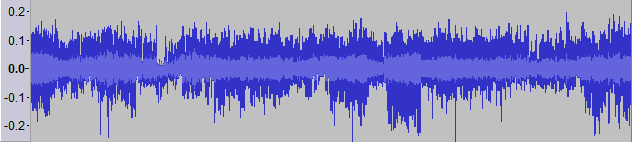
\includegraphics[width=1.0\textwidth]{../images/m5001_pred.png}
	\caption{Audio wave predicted by the model trained first on simple noised grooves, then on disc image.}
	\label{m5001_pred}
\end{figure}

\begin{figure}
	\centering
	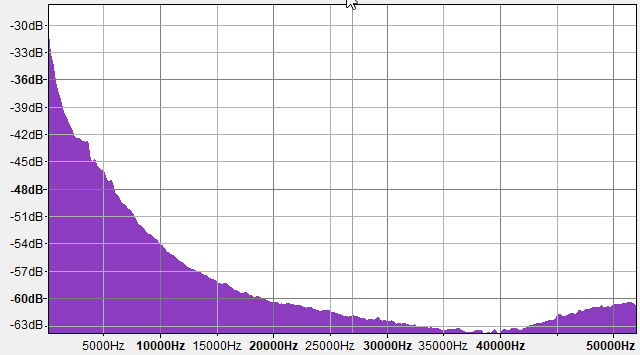
\includegraphics[width=0.8\textwidth]{../images/m5001_spectrum.png}
	\caption{Spectrum of the sound wave predicted by the model trained first on simple noised grooves, then on disc image.}
	\label{m5001_spectrum}
\end{figure}

Again, the results are not very good. When listening to the predicted sound, the singer can be heard, but there is a lot of noise on top of it.

It may be because of the misalignment of the goal audio wave regarding the groove track, or bad model hyper-parameters since the data is slightly different. It may also be that transfer learning is a bad idea for this problem, and the data are more different than it seems.

Our last hope for now is to train a new model only on disc images.
\subsection{Training new model}
The dataset preparation is exactly the same as for transfer learning. Creating a new model and training it can be tried immediately. Again, since the perfect alignment of goal audio and groove track is tricky, only one image is used at first to validate the models.

In order to account for the possible misalignment of the audio wave, the sliding window uses more lines of pixels : 21 now, against 15 before. Making the window even bigger would allow for more errors during alignment, but the model would need to learn to ignore a lot of lines that are far from the interesting ones. Furthermore, the window width is also increased from 320 to 360 pixels, as the track is sometimes quite off-center, and one of the edges is partially or entirely outside of the window.

Same as before, 15\% of the windows are ignored during training, and used for validation scoring.

As first fine-tuning, different learning rates are tried , from 1e-8 to 10 exponentially. All other parameters are kept the same as the best model from prototype 2.

After training for 3 times on the image, some values can already be removed for the possibilities : learning rates from 1e-2 to 10 prevents the model from learning anything. The MSE is stuck around 1.0 at all times for those learning rates, which is really bad considering that all our values are normalized.

The other versions are trained until epoch 6. However, none of them can produce a nice sound wave. They all predict a line close to 0 amplitude for some reason.

Also, it has come to attention that the distortion of the groove image due to the off-center hole causes the Weaver generated audio to be faster at certain places and slower at others when comparing with the tape version. A possible workaround would be to align the audio in smaller parts, but it would take a lot of time.

\section{Conclusion}
The ML4NR project was not able to improve the current disc image process for sound wave generation. However, it obtained promising results when dealing with a simplified version of the problem. It paves the road for future projects going in the same direction. Prototypes 1 and 2 showed that a CNN can quickly learn to find lateral movement in a groove image, even when it is noised. There is no reason this ability can't be used for actual disc images.

Better results can certainly be obtained with further fine-tuning. All hyper-parameters affect the others in some way, and finding the right combination deserves a project in itself.
\subsection{Personal conclusion}
I really liked working on the ML4NR project. I learned a lot regarding machine learning, and everything was interesting.

The working environment was good, as all researchers at the LBNL were very nice.

I sometimes felt overwhelmed by the amount of possibilities offered by machine learning techniques. Everything seemed doable, and I was lost at what to try. Fortunately, my supervisors and consultants guided me in the right direction every time.

A citation I found during my machine learning researches stuck with me : "Determining the topology/flavor/training method/hyper parameters for deep learning is a black art with not much theory to guide you."\cite{transfer2} 
\subsection{Future work}
Multiple leads on how to possibly obtain better results emerged during the project :
\begin{itemize}
	\item Generate a "better" artificial noise for simple grooves. Do a detailed analysis on the actual noise found on disc images, and replicate it on clean artificial groove images. For example, the Gaussian noise is mainly found on the edges and not on the entire image.
	\item Test other optimizers and their properties. Finding the right optimizer and its correct parameters depends on the other hyper-parameters, so it should be done last.
	\item Prepare a bigger real disc images dataset, with correctly aligned audio goal. This could be a project on its own, because a lot of manipulations need to be done case by case.
	\item Going into a completely different direction, the audio generation could be improved by removing the noise from disc images. Auto-encoders seem to have good results for this type of problem. It would also need a detailed analysis of the actual noise.
	\item Other neural networks can be tried on this problem, for example LSTM.
\end{itemize}

\section{Declaration of honor}
I, the undersigned Benoit Ruffray, hereby declare on my honor that this document is the result of my own work.
I certify that I have not cheated by means of plagiarism or any other forms of fraud.
All my information sources and all author citations have been clearly mentioned.
\bibliographystyle{unsrt}
\bibliography{cdc}

\begin{appendices}
	\section{Prototype 1}
	\subsection{Models and results}
	All models, results and parameters can be found on the Google Drive folder.
	
	\begin{figure}
		\centering
		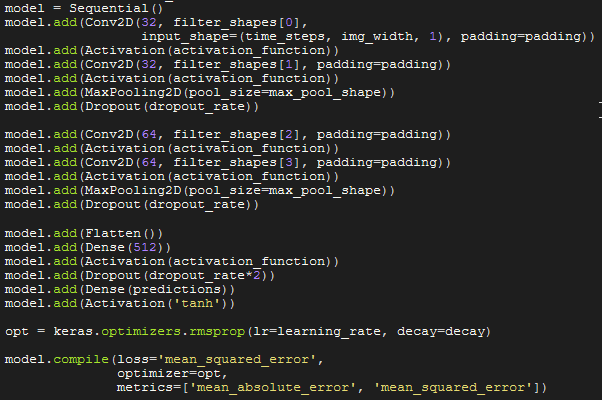
\includegraphics[width=0.8\textwidth]{../images/architecture_proto1.png}
		\caption{Code used to create models for prototype 1. All models follow this architecture.}
		\label{architecture_proto1}
	\end{figure}

	\begin{longtable} {|l|l|l|l|l|l|l|l|l|l|l|l|}		\hline
		Model & time & pred & conv & conv   & pool & pool   & drop & learn & decay & best & epoch \\
		name & steps &     & height & width & height & width & rate & rate & rate & MSE & \\ \hline
		\endhead
		model1 & 5 & 1 & 3 & 3 & 2 & 2 & 0.25 & 0.0001 & 1e-06 & 0.0069 & 1\\ \hline
		model2 & 5 & 1 & 3 & 5 & 2 & 2 & 0.25 & 0.0001 & 1e-06 & 0.0095 & 1\\ \hline
		model3 & 5 & 1 & 3 & 7 & 2 & 2 & 0.25 & 0.0001 & 1e-06 & 0.0088 & 1\\ \hline
		model4 & 5 & 1 & 3 & 9 & 2 & 2 & 0.25 & 0.0001 & 1e-06 & 0.0082 & 1\\ \hline
		model5 & 5 & 3 & 3 & 3 & 2 & 2 & 0.25 & 0.0001 & 1e-06 & 0.0196 & 1\\ \hline
		model6 & 5 & 3 & 3 & 5 & 2 & 2 & 0.25 & 0.0001 & 1e-06 & 0.0137 & 1\\ \hline
		model7 & 5 & 3 & 3 & 7 & 2 & 2 & 0.25 & 0.0001 & 1e-06 & 0.0147 & 1\\ \hline
		model8 & 5 & 3 & 3 & 9 & 2 & 2 & 0.25 & 0.0001 & 1e-06 & 0.0144 & 1\\ \hline
		model9 & 5 & 5 & 3 & 3 & 2 & 2 & 0.25 & 0.0001 & 1e-06 & 0.0298 & 1\\ \hline
		model10 & 5 & 5 & 3 & 5 & 2 & 2 & 0.25 & 0.0001 & 1e-06 & 0.0214 & 1\\ \hline
		model11 & 5 & 5 & 3 & 7 & 2 & 2 & 0.25 & 0.0001 & 1e-06 & 0.0242 & 1\\ \hline
		model12 & 5 & 5 & 3 & 9 & 2 & 2 & 0.25 & 0.0001 & 1e-06 & 0.0208 & 1\\ \hline
		model13 & 7 & 1 & 3 & 3 & 2 & 2 & 0.25 & 0.0001 & 1e-06 & 0.0244 & 1\\ \hline
		model14 & 7 & 1 & 3 & 5 & 2 & 2 & 0.25 & 0.0001 & 1e-06 & 0.0227 & 1\\ \hline
		model15 & 7 & 1 & 3 & 7 & 2 & 2 & 0.25 & 0.0001 & 1e-06 & 0.0343 & 1\\ \hline
		model16 & 7 & 1 & 3 & 9 & 2 & 2 & 0.25 & 0.0001 & 1e-06 & 0.0344 & 1\\ \hline
		model17 & 7 & 1 & 4 & 3 & 2 & 2 & 0.25 & 0.0001 & 1e-06 & 0.0215 & 1\\ \hline
		model18 & 7 & 1 & 4 & 5 & 2 & 2 & 0.25 & 0.0001 & 1e-06 & 0.0392 & 1\\ \hline
		model19 & 7 & 1 & 4 & 7 & 2 & 2 & 0.25 & 0.0001 & 1e-06 & 0.0356 & 1\\ \hline
		model20 & 7 & 1 & 4 & 9 & 2 & 2 & 0.25 & 0.0001 & 1e-06 & 0.0353 & 1\\ \hline
		model21 & 7 & 3 & 3 & 3 & 2 & 2 & 0.25 & 0.0001 & 1e-06 & 0.0383 & 1\\ \hline
		model22 & 7 & 3 & 3 & 5 & 2 & 2 & 0.25 & 0.0001 & 1e-06 & 0.0340 & 1\\ \hline
		model23 & 7 & 3 & 3 & 7 & 2 & 2 & 0.25 & 0.0001 & 1e-06 & 0.0385 & 1\\ \hline
		model24 & 7 & 3 & 3 & 9 & 2 & 2 & 0.25 & 0.0001 & 1e-06 & 0.0372 & 1\\ \hline
		model25 & 7 & 3 & 4 & 3 & 2 & 2 & 0.25 & 0.0001 & 1e-06 & 0.0349 & 1\\ \hline
		model26 & 7 & 3 & 4 & 5 & 2 & 2 & 0.25 & 0.0001 & 1e-06 & 0.0268 & 1\\ \hline
		model27 & 7 & 3 & 4 & 7 & 2 & 2 & 0.25 & 0.0001 & 1e-06 & 0.0350 & 1\\ \hline
		model28 & 7 & 3 & 4 & 9 & 2 & 2 & 0.25 & 0.0001 & 1e-06 & 0.0370 & 1\\ \hline
		model29 & 7 & 5 & 3 & 3 & 2 & 2 & 0.25 & 0.0001 & 1e-06 & 0.0424 & 1\\ \hline
		model30 & 7 & 5 & 3 & 5 & 2 & 2 & 0.25 & 0.0001 & 1e-06 & 0.0468 & 1\\ \hline
		model31 & 7 & 5 & 3 & 7 & 2 & 2 & 0.25 & 0.0001 & 1e-06 & 0.0415 & 1\\ \hline
		model32 & 7 & 5 & 3 & 9 & 2 & 2 & 0.25 & 0.0001 & 1e-06 & 0.0444 & 1\\ \hline
		model33 & 7 & 5 & 4 & 3 & 2 & 2 & 0.25 & 0.0001 & 1e-06 & 0.0412 & 1\\ \hline
		model34 & 7 & 5 & 4 & 5 & 2 & 2 & 0.25 & 0.0001 & 1e-06 & 0.0465 & 1\\ \hline
		model35 & 7 & 5 & 4 & 7 & 2 & 2 & 0.25 & 0.0001 & 1e-06 & 0.0437 & 1\\ \hline
		model36 & 7 & 5 & 4 & 9 & 2 & 2 & 0.25 & 0.0001 & 1e-06 & 0.0395 & 1\\ \hline
		model37 & 7 & 7 & 3 & 3 & 2 & 2 & 0.25 & 0.0001 & 1e-06 & 0.0577 & 1\\ \hline
		model38 & 7 & 7 & 3 & 5 & 2 & 2 & 0.25 & 0.0001 & 1e-06 & 0.0536 & 1\\ \hline
		model39 & 7 & 7 & 3 & 7 & 2 & 2 & 0.25 & 0.0001 & 1e-06 & 0.0561 & 1\\ \hline
		model40 & 7 & 7 & 3 & 9 & 2 & 2 & 0.25 & 0.0001 & 1e-06 & 0.0530 & 1\\ \hline
		model41 & 7 & 7 & 4 & 3 & 2 & 2 & 0.25 & 0.0001 & 1e-06 & 0.0510 & 1\\ \hline
		model42 & 7 & 7 & 4 & 5 & 2 & 2 & 0.25 & 0.0001 & 1e-06 & 0.0477 & 1\\ \hline
		model43 & 7 & 7 & 4 & 7 & 2 & 2 & 0.25 & 0.0001 & 1e-06 & 0.0571 & 1\\ \hline
		model44 & 7 & 7 & 4 & 9 & 2 & 2 & 0.25 & 0.0001 & 1e-06 & 0.0568 & 1\\ \hline
		model45 & 9 & 1 & 3 & 3 & 2 & 2 & 0.25 & 0.0001 & 1e-06 & 0.0288 & 1\\ \hline
		model46 & 9 & 1 & 3 & 5 & 2 & 2 & 0.25 & 0.0001 & 1e-06 & 0.0303 & 1\\ \hline
		model47 & 9 & 1 & 3 & 7 & 2 & 2 & 0.25 & 0.0001 & 1e-06 & 0.0344 & 1\\ \hline
		model48 & 9 & 1 & 3 & 9 & 2 & 2 & 0.25 & 0.0001 & 1e-06 & 0.0282 & 1\\ \hline
		model49 & 9 & 1 & 4 & 3 & 2 & 2 & 0.25 & 0.0001 & 1e-06 & 0.0270 & 1\\ \hline
		model50 & 9 & 1 & 4 & 5 & 2 & 2 & 0.25 & 0.0001 & 1e-06 & 0.0315 & 1\\ \hline
		model51 & 9 & 1 & 4 & 7 & 2 & 2 & 0.25 & 0.0001 & 1e-06 & 0.0285 & 1\\ \hline
		model52 & 9 & 1 & 4 & 9 & 2 & 2 & 0.25 & 0.0001 & 1e-06 & 0.0248 & 1\\ \hline
		model53 & 9 & 1 & 5 & 3 & 2 & 2 & 0.25 & 0.0001 & 1e-06 & 0.0242 & 1\\ \hline
	\end{longtable}
	
	
	\begin{longtable}{|l|l|l|l|l|l|l|l|l|l|l|l|}
		\hline
		Model & time & pred & conv & conv   & pool & pool   & drop & learn & decay & best & epoch \\
		name & steps &     & height & width & height & width & rate & rate & rate & MSE & \\ \hline
		model1000 & 5 & 1 & 3 & 3 & 1 & 1 & 0.0 & 0.0001 & 1e-06 & 0.0554 & 1\\ \hline
	\end{longtable}
	
	
	\subsection{Image dataset}
	\begin{longtable}{|l|}
			\hline
			Training dataset \\ \hline
			f110\_a10\_e3\_b12\_g160\_h80000.tif \\ \hline 
			f1150\_a10\_e3\_b12\_g160\_h80000.tif \\ \hline 
			f1155\_a10\_e3\_b12\_g160\_h80000.tif \\ \hline 
			f1305\_a10\_e3\_b12\_g160\_h80000.tif \\ \hline 
			f1355\_a10\_e3\_b12\_g160\_h80000.tif \\ \hline 
			f1400\_a10\_e3\_b12\_g160\_h80000.tif \\ \hline 
			f1480\_a10\_e3\_b12\_g160\_h80000.tif \\ \hline 
			f1510\_a10\_e3\_b12\_g160\_h80000.tif \\ \hline 
			f1765\_a10\_e3\_b12\_g160\_h80000.tif \\ \hline 
			f1815\_a10\_e3\_b12\_g160\_h80000.tif \\ \hline 
			f1875\_a10\_e3\_b12\_g160\_h80000.tif \\ \hline 
			f1935\_a10\_e3\_b12\_g160\_h80000.tif \\ \hline 
			f1955\_a10\_e3\_b12\_g160\_h80000.tif \\ \hline 
			f2035\_a10\_e3\_b12\_g160\_h80000.tif \\ \hline 
			f2075\_a10\_e3\_b12\_g160\_h80000.tif \\ \hline 
			f210\_a10\_e3\_b12\_g160\_h80000.tif \\ \hline 
			f2110\_a10\_e3\_b12\_g160\_h80000.tif \\ \hline 
			f2150\_a10\_e3\_b12\_g160\_h80000.tif \\ \hline 
			f2190\_a10\_e3\_b12\_g160\_h80000.tif \\ \hline 
			f2210\_a10\_e3\_b12\_g160\_h80000.tif \\ \hline 
			f2260\_a10\_e3\_b12\_g160\_h80000.tif \\ \hline 
			f2330\_a10\_e3\_b12\_g160\_h80000.tif \\ \hline 
			f235\_a10\_e3\_b12\_g160\_h80000.tif \\ \hline 
			f2390\_a10\_e3\_b12\_g160\_h80000.tif \\ \hline 
			f2420\_a10\_e3\_b12\_g160\_h80000.tif \\ \hline 
			f2470\_a10\_e3\_b12\_g160\_h80000.tif \\ \hline 
			f2490\_a10\_e3\_b12\_g160\_h80000.tif \\ \hline 
			f2580\_a10\_e3\_b12\_g160\_h80000.tif \\ \hline 
			f25\_a10\_e3\_b12\_g160\_h80000.tif \\ \hline 
			f2740\_a10\_e3\_b12\_g160\_h80000.tif \\ \hline 
			f2760\_a10\_e3\_b12\_g160\_h80000.tif \\ \hline 
			f2775\_a10\_e3\_b12\_g160\_h80000.tif \\ \hline 
			f3045\_a10\_e3\_b12\_g160\_h80000.tif \\ \hline 
			f3050\_a10\_e3\_b12\_g160\_h80000.tif \\ \hline 
			f3125\_a10\_e3\_b12\_g160\_h80000.tif \\ \hline 
			f3140\_a10\_e3\_b12\_g160\_h80000.tif \\ \hline 
			f3200\_a10\_e3\_b12\_g160\_h80000.tif \\ \hline 
			f3205\_a10\_e3\_b12\_g160\_h80000.tif \\ \hline 
			f3220\_a10\_e3\_b12\_g160\_h80000.tif \\ \hline 
			f3365\_a10\_e3\_b12\_g160\_h80000.tif \\ \hline 
			f3405\_a10\_e3\_b12\_g160\_h80000.tif \\ \hline 
			f350\_a10\_e3\_b12\_g160\_h80000.tif \\ \hline 
			f3530\_a10\_e3\_b12\_g160\_h80000.tif \\ \hline 
			f3790\_a10\_e3\_b12\_g160\_h80000.tif \\ \hline 
			f3795\_a10\_e3\_b12\_g160\_h80000.tif \\ \hline 
			f3810\_a10\_e3\_b12\_g160\_h80000.tif \\ \hline 
			f3820\_a10\_e3\_b12\_g160\_h80000.tif \\ \hline 
			f3825\_a10\_e3\_b12\_g160\_h80000.tif \\ \hline 
			f3900\_a10\_e3\_b12\_g160\_h80000.tif \\ \hline 
			f3935\_a10\_e3\_b12\_g160\_h80000.tif \\ \hline 
			f3940\_a10\_e3\_b12\_g160\_h80000.tif \\ \hline 
			f4055\_a10\_e3\_b12\_g160\_h80000.tif \\ \hline 
			f4060\_a10\_e3\_b12\_g160\_h80000.tif \\ \hline 
			f4215\_a10\_e3\_b12\_g160\_h80000.tif \\ \hline 
			f435\_a10\_e3\_b12\_g160\_h80000.tif \\ \hline 
			f4390\_a10\_e3\_b12\_g160\_h80000.tif \\ \hline 
			f4505\_a10\_e3\_b12\_g160\_h80000.tif \\ \hline 
			f4670\_a10\_e3\_b12\_g160\_h80000.tif \\ \hline 
			f4780\_a10\_e3\_b12\_g160\_h80000.tif \\ \hline 
			f4785\_a10\_e3\_b12\_g160\_h80000.tif \\ \hline 
			f4875\_a10\_e3\_b12\_g160\_h80000.tif \\ \hline 
			f4885\_a10\_e3\_b12\_g160\_h80000.tif \\ \hline 
			f4950\_a10\_e3\_b12\_g160\_h80000.tif \\ \hline 
			f4955\_a10\_e3\_b12\_g160\_h80000.tif \\ \hline 
			f4990\_a10\_e3\_b12\_g160\_h80000.tif \\ \hline 
			f50\_a10\_e3\_b12\_g160\_h80000.tif \\ \hline 
			f510\_a10\_e3\_b12\_g160\_h80000.tif \\ \hline 
			f545\_a10\_e3\_b12\_g160\_h80000.tif \\ \hline 
			f555\_a10\_e3\_b12\_g160\_h80000.tif \\ \hline 
			f595\_a10\_e3\_b12\_g160\_h80000.tif \\ \hline 
			f600\_a10\_e3\_b12\_g160\_h80000.tif \\ \hline 
			f650\_a10\_e3\_b12\_g160\_h80000.tif \\ \hline 
			f710\_a10\_e3\_b12\_g160\_h80000.tif \\ \hline 
			f75\_a10\_e3\_b12\_g160\_h80000.tif \\ \hline 
			f765\_a10\_e3\_b12\_g160\_h80000.tif \\ \hline 
			f905\_a10\_e3\_b12\_g160\_h80000.tif \\ \hline 
			f925\_a10\_e3\_b12\_g160\_h80000.tif \\ \hline 
			f975\_a10\_e3\_b12\_g160\_h80000.tif \\ \hline 
		\caption{Training dataset of prototype 1}
		\label{proto1_train}
	\end{longtable}
	Each file name contains the parameters used to generate it in the Weaver plugin. For example, f1875\_a10\_e3\_b12\_g160\_h80000.tif is a groove of frequency 1875 Hz, amplitude 10, edge width 3, bottom width 12, groove width 160, and 80'000 pixels of height.
	
	\begin{longtable}{|l|}
		\hline
		Testing dataset \\ \hline 
		f1550\_a10\_e3\_b12\_g160\_h80000.tif \\ \hline 
		f2100\_a10\_e3\_b12\_g160\_h80000.tif \\ \hline 
		f2175\_a10\_e3\_b12\_g160\_h80000.tif \\ \hline 
		f2375\_a10\_e3\_b12\_g160\_h80000.tif \\ \hline 
		f2695\_a10\_e3\_b12\_g160\_h80000.tif \\ \hline 
		f2865\_a10\_e3\_b12\_g160\_h80000.tif \\ \hline 
		f3170\_a10\_e3\_b12\_g160\_h80000.tif \\ \hline 
		f3255\_a10\_e3\_b12\_g160\_h80000.tif \\ \hline 
		f3540\_a10\_e3\_b12\_g160\_h80000.tif \\ \hline 
		f3875\_a10\_e3\_b12\_g160\_h80000.tif \\ \hline 
		f405\_a10\_e3\_b12\_g160\_h80000.tif \\ \hline 
		f4200\_a10\_e3\_b12\_g160\_h80000.tif \\ \hline 
		f4580\_a10\_e3\_b12\_g160\_h80000.tif \\ \hline 
		f4845\_a10\_e3\_b12\_g160\_h80000.tif \\ \hline 
		f4960\_a10\_e3\_b12\_g160\_h80000.tif \\ \hline 
		f60\_a10\_e3\_b12\_g160\_h80000.tif \\ \hline 
		f620\_a10\_e3\_b12\_g160\_h80000.tif \\ \hline 
		f965\_a10\_e3\_b12\_g160\_h80000.tif \\ \hline
		\caption{Testing dataset of prototype 1}
		\label{proto1_test}
	\end{longtable}

	
	\section{Prototype 2}
	\subsection{Models and results}
	All models, results and parameters can be found on the Google Drive folder.
	
	\begin{longtable}{|l|l|l|l|l|l|l|l|l|l|l|l|}
		\hline
		Model & time & pred & conv & conv   & pool & pool   & drop & learn & decay & best & epoch \\
		name & steps &     & height & width & height & width & rate & rate & rate & MSE & \\ \hline
		\endhead
		model3000 & 5 & 1 & 3 & 3 & 2 & 2 & 0.25 & 0.0001 & 1e-06 & 0.0311 & 5\\ \hline
		model3001 & 5 & 1 & 3 & 3 & 2 & 2 & 0.25 & 0.001 & 1e-05 & 0.0321 & 1\\ \hline
		model3002 & 5 & 1 & 3 & 3 & 2 & 2 & 0.25 & 0.001 & 0.0 & 0.0387 & 5\\ \hline
		model3003 & 15 & 1 & 3 & 3 & 2 & 2 & 0.25 & 0.001 & 0.0 & 0.0254 & 4\\ \hline
		model3004 & 9 & 1 & 3 & 3 & 2 & 2 & 0.25 & 0.001 & 0.0 & 0.0323 & 1\\ \hline
	\end{longtable}

\begin{longtable}{|l|l|l|l|l|l|l|l|l|l|l|l|}
	\hline
	Model & time & pred & conv & conv   & pool & pool   & drop & learn & decay & best & epoch \\
	name & steps &     & height & width & height & width & rate & rate & rate & MSE & \\ \hline
	\endhead
	model4000 & 15 & 1 & 3 & 3 & 2 & 2 & 0.25 & 0.001 & 0.0 & 0.0287 & 5\\ \hline
	model4001 & 5 & 1 & 3 & 3 & 2 & 2 & 0.25 & 0.001 & 0.0 & 0.0405 & 0.8\\ \hline
	model4002 & 15 & 1 & 3 & 3 & 2 & 2 & 0.25 & 0.001 & 0.0 & 0.0268 & 1\\ \hline
	model4003 & 15 & 1 & 3 & 3 & 2 & 2 & 0.25 & 0.01 & 0.0 & 1.5004 & 0.1\\ \hline
	model4004 & 15 & 1 & 3 & 3 & 2 & 2 & 0.25 & 0.001 & 0.0 & 0.0172 & 2.6\\ \hline
	model4005 & 5 & 1 & 3 & 3 & 2 & 2 & 0.25 & 0.001 & 0.0 & 0.0346 & 1.6\\ \hline
	model4006 & 25 & 1 & 3 & 3 & 2 & 2 & 0.25 & 0.001 & 0.0 & 0.0294 & 0.1\\ \hline
\end{longtable}

	
	\subsection{Image dataset}
	\begin{longtable}{|l|}
		\hline
		Testing dataset \\ \hline 
		f1140\_a10\_e4\_b10\_g160\_h80000.tif \\ \hline 
		f1294\_a10\_e2\_b10\_g150\_h80000.tif \\ \hline 
		f1530\_a10\_e2\_b10\_g155\_h80000.tif \\ \hline 
		f1681\_a10\_e3\_b13\_g150\_h80000.tif \\ \hline 
		f173\_a10\_e3\_b13\_g165\_h80000.tif \\ \hline 
		f1862\_a10\_e3\_b13\_g165\_h80000.tif \\ \hline 
		f1976\_a10\_e2\_b12\_g165\_h80000.tif \\ \hline 
		f2042\_a10\_e2\_b12\_g160\_h80000.tif \\ \hline 
		f2161\_a10\_e3\_b10\_g160\_h80000.tif \\ \hline 
		f2426\_a10\_e2\_b10\_g150\_h80000.tif \\ \hline 
		f2626\_a10\_e4\_b13\_g150\_h80000.tif \\ \hline 
		f2709\_a10\_e3\_b11\_g165\_h80000.tif \\ \hline 
		f2905\_a10\_e3\_b11\_g165\_h80000.tif \\ \hline 
		f294\_a10\_e3\_b10\_g165\_h80000.tif \\ \hline 
		f31\_a10\_e4\_b12\_g150\_h80000.tif \\ \hline 
		f3202\_a10\_e3\_b11\_g160\_h80000.tif \\ \hline 
		f3411\_a10\_e3\_b10\_g160\_h80000.tif \\ \hline 
		f3577\_a10\_e4\_b12\_g155\_h80000.tif \\ \hline 
		f3817\_a10\_e4\_b12\_g155\_h80000.tif \\ \hline 
		f3968\_a10\_e4\_b12\_g165\_h80000.tif \\ \hline 
		f4070\_a10\_e4\_b12\_g155\_h80000.tif \\ \hline 
		f426\_a10\_e4\_b11\_g155\_h80000.tif \\ \hline 
		f4299\_a10\_e2\_b11\_g160\_h80000.tif \\ \hline 
		f4452\_a10\_e4\_b13\_g150\_h80000.tif \\ \hline 
		f4560\_a10\_e4\_b13\_g160\_h80000.tif \\ \hline 
		f4742\_a10\_e2\_b10\_g160\_h80000.tif \\ \hline 
		f4880\_a10\_e4\_b11\_g150\_h80000.tif \\ \hline 
		f610\_a10\_e4\_b13\_g165\_h80000.tif \\ \hline 
		f673\_a10\_e2\_b13\_g155\_h80000.tif \\ \hline 
		f862\_a10\_e2\_b13\_g160\_h80000.tif \\ \hline 
	\end{longtable}
	
	\begin{longtable}{|l|}
		\hline
		Training dataset \\ \hline 
		f1034\_a10\_e2\_b13\_g150\_h80000.tif \\ \hline 
		f1036\_a10\_e2\_b12\_g150\_h80000.tif \\ \hline 
		f1043\_a10\_e2\_b13\_g165\_h80000.tif \\ \hline 
		f1159\_a10\_e2\_b10\_g165\_h80000.tif \\ \hline 
		f1227\_a10\_e2\_b10\_g155\_h80000.tif \\ \hline 
		f1231\_a10\_e2\_b10\_g155\_h80000.tif \\ \hline 
		f1236\_a10\_e4\_b13\_g155\_h80000.tif \\ \hline 
		f1245\_a10\_e4\_b13\_g150\_h80000.tif \\ \hline 
		f1286\_a10\_e4\_b13\_g155\_h80000.tif \\ \hline 
		f1327\_a10\_e2\_b13\_g155\_h80000.tif \\ \hline 
		f1356\_a10\_e2\_b11\_g165\_h80000.tif \\ \hline 
		f1385\_a10\_e3\_b11\_g165\_h80000.tif \\ \hline 
		f144\_a10\_e2\_b10\_g150\_h80000.tif \\ \hline 
		f1492\_a10\_e2\_b12\_g155\_h80000.tif \\ \hline 
		f150\_a10\_e3\_b12\_g160\_h80000.tif \\ \hline 
		f1519\_a10\_e4\_b12\_g150\_h80000.tif \\ \hline 
		f1522\_a10\_e2\_b13\_g165\_h80000.tif \\ \hline 
		f158\_a10\_e4\_b11\_g165\_h80000.tif \\ \hline 
		f1612\_a10\_e2\_b10\_g155\_h80000.tif \\ \hline 
		f1643\_a10\_e2\_b13\_g165\_h80000.tif \\ \hline 
		f1645\_a10\_e2\_b11\_g165\_h80000.tif \\ \hline 
		f1660\_a10\_e2\_b11\_g155\_h80000.tif \\ \hline 
		f1667\_a10\_e3\_b11\_g155\_h80000.tif \\ \hline 
		f1675\_a10\_e3\_b13\_g155\_h80000.tif \\ \hline 
		f1742\_a10\_e4\_b11\_g150\_h80000.tif \\ \hline 
		f177\_a10\_e4\_b12\_g160\_h80000.tif \\ \hline 
		f1784\_a10\_e3\_b12\_g165\_h80000.tif \\ \hline 
		f1802\_a10\_e2\_b13\_g150\_h80000.tif \\ \hline 
		f1802\_a10\_e4\_b13\_g160\_h80000.tif \\ \hline 
		f1818\_a10\_e3\_b12\_g150\_h80000.tif \\ \hline 
		f1842\_a10\_e2\_b11\_g165\_h80000.tif \\ \hline 
		f1927\_a10\_e2\_b12\_g160\_h80000.tif \\ \hline 
		f1934\_a10\_e3\_b11\_g165\_h80000.tif \\ \hline 
		f1975\_a10\_e4\_b10\_g165\_h80000.tif \\ \hline 
		f1977\_a10\_e4\_b13\_g165\_h80000.tif \\ \hline 
		f1996\_a10\_e4\_b13\_g150\_h80000.tif \\ \hline 
		f2081\_a10\_e4\_b11\_g150\_h80000.tif \\ \hline 
		f2084\_a10\_e3\_b10\_g160\_h80000.tif \\ \hline 
		f2085\_a10\_e2\_b11\_g165\_h80000.tif \\ \hline 
		f2096\_a10\_e3\_b13\_g150\_h80000.tif \\ \hline 
		f2148\_a10\_e2\_b13\_g150\_h80000.tif \\ \hline 
		f2156\_a10\_e4\_b10\_g150\_h80000.tif \\ \hline 
		f2204\_a10\_e2\_b10\_g150\_h80000.tif \\ \hline 
		f220\_a10\_e3\_b12\_g155\_h80000.tif \\ \hline 
		f2220\_a10\_e2\_b12\_g155\_h80000.tif \\ \hline 
		f2236\_a10\_e3\_b10\_g155\_h80000.tif \\ \hline 
		f2239\_a10\_e4\_b13\_g165\_h80000.tif \\ \hline 
		f2319\_a10\_e4\_b12\_g150\_h80000.tif \\ \hline 
		f2384\_a10\_e3\_b10\_g150\_h80000.tif \\ \hline 
		f2426\_a10\_e4\_b11\_g160\_h80000.tif \\ \hline 
		f2438\_a10\_e3\_b12\_g160\_h80000.tif \\ \hline 
		f2461\_a10\_e2\_b11\_g155\_h80000.tif \\ \hline 
		f2475\_a10\_e3\_b12\_g160\_h80000.tif \\ \hline 
		f2479\_a10\_e4\_b11\_g165\_h80000.tif \\ \hline 
		f247\_a10\_e2\_b12\_g165\_h80000.tif \\ \hline 
		f2530\_a10\_e3\_b10\_g155\_h80000.tif \\ \hline 
		f2630\_a10\_e3\_b12\_g160\_h80000.tif \\ \hline 
		f2642\_a10\_e3\_b13\_g150\_h80000.tif \\ \hline 
		f2672\_a10\_e4\_b11\_g155\_h80000.tif \\ \hline 
		f2673\_a10\_e4\_b12\_g150\_h80000.tif \\ \hline 
		f2695\_a10\_e2\_b10\_g155\_h80000.tif \\ \hline 
		f2708\_a10\_e2\_b13\_g160\_h80000.tif \\ \hline 
		f272\_a10\_e2\_b10\_g150\_h80000.tif \\ \hline 
		f273\_a10\_e3\_b13\_g160\_h80000.tif \\ \hline 
		f2811\_a10\_e4\_b12\_g165\_h80000.tif \\ \hline 
		f2816\_a10\_e3\_b11\_g160\_h80000.tif \\ \hline 
		f2827\_a10\_e4\_b10\_g160\_h80000.tif \\ \hline 
		f2829\_a10\_e2\_b10\_g165\_h80000.tif \\ \hline 
		f2878\_a10\_e4\_b13\_g150\_h80000.tif \\ \hline 
		f2889\_a10\_e2\_b11\_g155\_h80000.tif \\ \hline 
		f291\_a10\_e4\_b11\_g165\_h80000.tif \\ \hline 
		f2971\_a10\_e2\_b13\_g150\_h80000.tif \\ \hline 
		f2977\_a10\_e2\_b13\_g165\_h80000.tif \\ \hline 
		f3004\_a10\_e2\_b10\_g160\_h80000.tif \\ \hline 
		f3029\_a10\_e3\_b10\_g165\_h80000.tif \\ \hline 
		f3055\_a10\_e2\_b11\_g160\_h80000.tif \\ \hline 
		f3129\_a10\_e2\_b12\_g165\_h80000.tif \\ \hline 
		f3280\_a10\_e2\_b13\_g165\_h80000.tif \\ \hline 
		f3292\_a10\_e4\_b11\_g165\_h80000.tif \\ \hline 
		f3307\_a10\_e3\_b11\_g150\_h80000.tif \\ \hline 
		f3318\_a10\_e2\_b11\_g155\_h80000.tif \\ \hline 
		f3348\_a10\_e3\_b11\_g155\_h80000.tif \\ \hline 
		f3383\_a10\_e4\_b11\_g155\_h80000.tif \\ \hline 
		f3415\_a10\_e2\_b13\_g155\_h80000.tif \\ \hline 
		f3426\_a10\_e3\_b12\_g165\_h80000.tif \\ \hline 
		f3428\_a10\_e4\_b12\_g150\_h80000.tif \\ \hline 
		f3436\_a10\_e3\_b10\_g150\_h80000.tif \\ \hline 
		f3473\_a10\_e3\_b13\_g160\_h80000.tif \\ \hline 
		f3522\_a10\_e2\_b13\_g150\_h80000.tif \\ \hline 
		f3605\_a10\_e4\_b13\_g160\_h80000.tif \\ \hline 
		f3729\_a10\_e2\_b12\_g160\_h80000.tif \\ \hline 
		f3734\_a10\_e3\_b11\_g165\_h80000.tif \\ \hline 
		f3737\_a10\_e4\_b13\_g155\_h80000.tif \\ \hline 
		f374\_a10\_e3\_b12\_g155\_h80000.tif \\ \hline 
		f3754\_a10\_e4\_b10\_g160\_h80000.tif \\ \hline 
		f3790\_a10\_e2\_b10\_g160\_h80000.tif \\ \hline 
		f385\_a10\_e3\_b11\_g150\_h80000.tif \\ \hline 
		f3903\_a10\_e4\_b13\_g155\_h80000.tif \\ \hline 
		f3904\_a10\_e3\_b13\_g165\_h80000.tif \\ \hline 
		f3905\_a10\_e3\_b12\_g155\_h80000.tif \\ \hline 
		f3927\_a10\_e3\_b11\_g165\_h80000.tif \\ \hline 
		f3930\_a10\_e2\_b10\_g165\_h80000.tif \\ \hline 
		f3938\_a10\_e4\_b10\_g155\_h80000.tif \\ \hline 
		f398\_a10\_e2\_b11\_g165\_h80000.tif \\ \hline 
		f4017\_a10\_e2\_b10\_g165\_h80000.tif \\ \hline 
		f4026\_a10\_e2\_b11\_g165\_h80000.tif \\ \hline 
		f4040\_a10\_e3\_b13\_g160\_h80000.tif \\ \hline 
		f4056\_a10\_e4\_b10\_g165\_h80000.tif \\ \hline 
		f4063\_a10\_e2\_b12\_g155\_h80000.tif \\ \hline 
		f4069\_a10\_e2\_b12\_g150\_h80000.tif \\ \hline 
		f4072\_a10\_e3\_b12\_g155\_h80000.tif \\ \hline 
		f4094\_a10\_e2\_b13\_g150\_h80000.tif \\ \hline 
		f409\_a10\_e2\_b12\_g160\_h80000.tif \\ \hline 
		f415\_a10\_e2\_b10\_g160\_h80000.tif \\ \hline 
		f4179\_a10\_e2\_b12\_g150\_h80000.tif \\ \hline 
		f4184\_a10\_e2\_b13\_g165\_h80000.tif \\ \hline 
		f420\_a10\_e2\_b10\_g150\_h80000.tif \\ \hline 
		f4242\_a10\_e4\_b13\_g150\_h80000.tif \\ \hline 
		f4243\_a10\_e4\_b11\_g150\_h80000.tif \\ \hline 
		f4320\_a10\_e3\_b13\_g160\_h80000.tif \\ \hline 
		f4328\_a10\_e3\_b13\_g165\_h80000.tif \\ \hline 
		f4345\_a10\_e3\_b13\_g155\_h80000.tif \\ \hline 
		f4366\_a10\_e4\_b13\_g155\_h80000.tif \\ \hline 
		f4388\_a10\_e2\_b11\_g150\_h80000.tif \\ \hline 
		f4410\_a10\_e4\_b12\_g160\_h80000.tif \\ \hline 
		f4459\_a10\_e4\_b13\_g165\_h80000.tif \\ \hline 
		f4476\_a10\_e2\_b10\_g165\_h80000.tif \\ \hline 
		f4499\_a10\_e2\_b11\_g165\_h80000.tif \\ \hline 
		f4512\_a10\_e3\_b10\_g155\_h80000.tif \\ \hline 
		f4534\_a10\_e4\_b11\_g155\_h80000.tif \\ \hline 
		f4551\_a10\_e4\_b10\_g160\_h80000.tif \\ \hline 
		f4611\_a10\_e2\_b11\_g160\_h80000.tif \\ \hline 
		f4650\_a10\_e2\_b11\_g150\_h80000.tif \\ \hline 
		f4700\_a10\_e2\_b13\_g160\_h80000.tif \\ \hline 
		f4711\_a10\_e2\_b10\_g165\_h80000.tif \\ \hline 
		f4740\_a10\_e2\_b12\_g160\_h80000.tif \\ \hline 
		f4740\_a10\_e2\_b12\_g165\_h80000.tif \\ \hline 
		f4745\_a10\_e2\_b13\_g165\_h80000.tif \\ \hline 
		f4750\_a10\_e4\_b10\_g165\_h80000.tif \\ \hline 
		f4771\_a10\_e3\_b10\_g165\_h80000.tif \\ \hline 
		f4771\_a10\_e4\_b12\_g155\_h80000.tif \\ \hline 
		f4772\_a10\_e4\_b11\_g165\_h80000.tif \\ \hline 
		f4779\_a10\_e4\_b10\_g160\_h80000.tif \\ \hline 
		f47\_a10\_e3\_b10\_g150\_h80000.tif \\ \hline 
		f485\_a10\_e2\_b13\_g160\_h80000.tif \\ \hline 
		f4969\_a10\_e3\_b13\_g165\_h80000.tif \\ \hline 
		f4977\_a10\_e2\_b10\_g155\_h80000.tif \\ \hline 
		f4978\_a10\_e4\_b12\_g150\_h80000.tif \\ \hline 
		f497\_a10\_e4\_b12\_g155\_h80000.tif \\ \hline 
		f528\_a10\_e2\_b12\_g155\_h80000.tif \\ \hline 
		f533\_a10\_e3\_b13\_g155\_h80000.tif \\ \hline 
		f558\_a10\_e3\_b13\_g150\_h80000.tif \\ \hline 
		f604\_a10\_e3\_b13\_g155\_h80000.tif \\ \hline 
		f616\_a10\_e4\_b11\_g150\_h80000.tif \\ \hline 
		f617\_a10\_e3\_b11\_g160\_h80000.tif \\ \hline 
		f645\_a10\_e3\_b11\_g155\_h80000.tif \\ \hline 
		f666\_a10\_e4\_b11\_g160\_h80000.tif \\ \hline 
		f666\_a10\_e4\_b13\_g155\_h80000.tif \\ \hline 
		f671\_a10\_e2\_b10\_g155\_h80000.tif \\ \hline 
		f678\_a10\_e3\_b11\_g150\_h80000.tif \\ \hline 
		f705\_a10\_e2\_b11\_g160\_h80000.tif \\ \hline 
		f728\_a10\_e2\_b11\_g160\_h80000.tif \\ \hline 
		f754\_a10\_e4\_b13\_g160\_h80000.tif \\ \hline 
		f77\_a10\_e3\_b10\_g160\_h80000.tif \\ \hline 
		f827\_a10\_e4\_b13\_g160\_h80000.tif \\ \hline 
		f84\_a10\_e2\_b13\_g165\_h80000.tif \\ \hline 
		f853\_a10\_e3\_b11\_g165\_h80000.tif \\ \hline 
		f870\_a10\_e2\_b13\_g150\_h80000.tif \\ \hline 
		f874\_a10\_e2\_b13\_g160\_h80000.tif \\ \hline 
		f942\_a10\_e3\_b12\_g165\_h80000.tif \\ \hline 
	\end{longtable}
	
	\section{Prototype 3 and 4}
	\subsection{Models and results}
	All models, results and parameters can be found on the Google Drive folder.
	
	Model 5000 : train only on artificial images
	
	Model 5002+ : train only on disc, fin tune window height, dropout rate, learning rate.
	
	Model 6001+ : fine tuning Adam optimizer 
	
	\begin{longtable}{|l|l|l|l|l|l|l|l|l|l|l|l|}
		\hline
		Model & time & pred & conv & conv   & pool & pool   & drop & learn & decay & best & epoch \\
		name & steps &     & height & width & height & width & rate & rate & rate & MSE & \\ \hline
		\endhead
		model5000 & 15 & 1 & 3 & 3 & 2 & 2 & [0.25, 0.25, 0.5] & 0.001 & 0.0 & 0.0000 & 0\\ \hline
		model5002 & 15 & 1 & 3 & 3 & 2 & 2 & [0.25, 0.25, 0.5] & 0.001 & 0.0 & 0.0000 & 0\\ \hline
		model5003 & 25 & 1 & 3 & 3 & 2 & 2 & [0.25, 0.25, 0.5] & 0.001 & 0.0 & 0.0000 & 0\\ \hline
		model5004 & 15 & 1 & 3 & 3 & 2 & 2 & [0.5, 0.5, 0.7] & 1 & 0.0 & 0.0000 & 0\\ \hline
		model5005 & 21 & 1 & 3 & 3 & 2 & 2 & [0.5, 0.5, 0.7] & 0.0005 & 1e-06 & 0.0000 & 0\\ \hline
	\end{longtable}
	
	
	\begin{longtable}{|l|l|l|l|l|l|l|l|l|l|l|l|}
		\hline
		Model & time & pred & conv & conv   & pool & pool   & drop & learn & decay & best & epoch \\
		name & steps &     & height & width & height & width & rate & rate & rate & MSE & \\ \hline
		\endhead
		model6001 & 21 & 1 & 3 & 3 & 2 & 2 & [0.25, 0.5, 0.5] & 1e-08 & 0 & 0.0361 & 4\\ \hline
		model6002 & 21 & 1 & 3 & 3 & 2 & 2 & [0.25, 0.5, 0.5] & 1e-07 & 0 & 0.0354 & 1\\ \hline
		model6003 & 21 & 1 & 3 & 3 & 2 & 2 & [0.25, 0.5, 0.5] & 1e-06 & 0 & 0.0355 & 1\\ \hline
		model6004 & 21 & 1 & 3 & 3 & 2 & 2 & [0.25, 0.5, 0.5] & 1e-05 & 0 & 0.0376 & 1\\ \hline
		model6005 & 21 & 1 & 3 & 3 & 2 & 2 & [0.25, 0.5, 0.5] & 0.0001 & 0 & 0.0391 & 1\\ \hline
		model6006 & 21 & 1 & 3 & 3 & 2 & 2 & [0.25, 0.5, 0.5] & 0.001 & 0 & 0.0353 & 3\\ \hline
		model6007 & 21 & 1 & 3 & 3 & 2 & 2 & [0.25, 0.5, 0.5] & 0.01 & 0 & 1.0298 & 1\\ \hline
		model6008 & 21 & 1 & 3 & 3 & 2 & 2 & [0.25, 0.5, 0.5] & 0.1 & 0 & 1.0298 & 1\\ \hline
		model6009 & 21 & 1 & 3 & 3 & 2 & 2 & [0.25, 0.5, 0.5] & 1 & 0 & 1.0299 & 1\\ \hline
		model6010 & 21 & 1 & 3 & 3 & 2 & 2 & [0.25, 0.5, 0.5] & 10 & 0 & 1.0298 & 1\\ \hline
	\end{longtable}
	
	\subsection{Image dataset}
	Disc image : Johnny-52211.bmp
	\begin{longtable}{|l|}
		\hline
		Testing dataset \\ \hline 
		f1080\_a15\_e13\_b10\_g237\_h80000.tif \\ \hline 
		f1400\_a14\_e12\_b10\_g239\_h80000.tif \\ \hline 
		f1660\_a12\_e14\_b10\_g241\_h80000.tif \\ \hline 
		f1850\_a14\_e12\_b11\_g241\_h80000.tif \\ \hline 
		f220\_a14\_e14\_b10\_g237\_h80000.tif \\ \hline 
		f2250\_a13\_e14\_b10\_g243\_h80000.tif \\ \hline 
		f2720\_a17\_e14\_b10\_g239\_h80000.tif \\ \hline 
		f3600\_a15\_e12\_b11\_g235\_h80000.tif \\ \hline 
		f3800\_a13\_e13\_b10\_g239\_h80000.tif \\ \hline 
		f4020\_a15\_e14\_b10\_g235\_h80000.tif \\ \hline 
		f4360\_a15\_e14\_b10\_g241\_h80000.tif \\ \hline 
		f4650\_a18\_e12\_b11\_g239\_h80000.tif \\ \hline 
		f4860\_a15\_e12\_b10\_g241\_h80000.tif \\ \hline 
		f570\_a17\_e12\_b11\_g243\_h80000.tif \\ \hline 
		f840\_a16\_e13\_b11\_g241\_h80000.tif \\ \hline 
	\end{longtable}
	\begin{longtable}{|l|}
		\hline
		Training dataset \\ \hline 
		f1050\_a16\_e14\_b11\_g235\_h80000.tif \\ \hline 
		f1070\_a17\_e12\_b10\_g239\_h80000.tif \\ \hline 
		f1100\_a16\_e12\_b10\_g239\_h80000.tif \\ \hline 
		f1110\_a18\_e12\_b11\_g243\_h80000.tif \\ \hline 
		f1210\_a17\_e13\_b10\_g235\_h80000.tif \\ \hline 
		f1280\_a11\_e13\_b10\_g243\_h80000.tif \\ \hline 
		f1420\_a19\_e13\_b10\_g243\_h80000.tif \\ \hline 
		f1530\_a16\_e13\_b11\_g239\_h80000.tif \\ \hline 
		f1590\_a10\_e13\_b11\_g239\_h80000.tif \\ \hline 
		f1600\_a16\_e13\_b11\_g235\_h80000.tif \\ \hline 
		f1690\_a11\_e14\_b11\_g237\_h80000.tif \\ \hline 
		f1720\_a11\_e12\_b11\_g237\_h80000.tif \\ \hline 
		f1720\_a17\_e13\_b10\_g241\_h80000.tif \\ \hline 
		f1770\_a12\_e12\_b10\_g241\_h80000.tif \\ \hline 
		f1810\_a16\_e14\_b10\_g237\_h80000.tif \\ \hline 
		f1880\_a19\_e13\_b10\_g243\_h80000.tif \\ \hline 
		f1950\_a16\_e12\_b11\_g239\_h80000.tif \\ \hline 
		f1960\_a14\_e14\_b11\_g235\_h80000.tif \\ \hline 
		f1980\_a19\_e14\_b11\_g237\_h80000.tif \\ \hline 
		f2010\_a11\_e14\_b11\_g243\_h80000.tif \\ \hline 
		f2230\_a13\_e14\_b10\_g241\_h80000.tif \\ \hline 
		f2240\_a15\_e14\_b10\_g235\_h80000.tif \\ \hline 
		f2320\_a15\_e12\_b11\_g243\_h80000.tif \\ \hline 
		f2340\_a16\_e12\_b11\_g241\_h80000.tif \\ \hline 
		f2340\_a16\_e14\_b11\_g239\_h80000.tif \\ \hline 
		f2360\_a13\_e12\_b11\_g241\_h80000.tif \\ \hline 
		f240\_a16\_e14\_b11\_g243\_h80000.tif \\ \hline 
		f2420\_a15\_e12\_b11\_g239\_h80000.tif \\ \hline 
		f2450\_a19\_e12\_b10\_g237\_h80000.tif \\ \hline 
		f2510\_a15\_e13\_b11\_g235\_h80000.tif \\ \hline 
		f2690\_a11\_e14\_b10\_g239\_h80000.tif \\ \hline 
		f2690\_a16\_e13\_b10\_g239\_h80000.tif \\ \hline 
		f270\_a11\_e13\_b11\_g235\_h80000.tif \\ \hline 
		f280\_a19\_e13\_b10\_g237\_h80000.tif \\ \hline 
		f3020\_a13\_e14\_b10\_g241\_h80000.tif \\ \hline 
		f3110\_a16\_e14\_b11\_g237\_h80000.tif \\ \hline 
		f3160\_a17\_e13\_b11\_g243\_h80000.tif \\ \hline 
		f3220\_a16\_e13\_b10\_g235\_h80000.tif \\ \hline 
		f3290\_a15\_e12\_b10\_g243\_h80000.tif \\ \hline 
		f3450\_a19\_e13\_b10\_g243\_h80000.tif \\ \hline 
		f350\_a13\_e14\_b10\_g241\_h80000.tif \\ \hline 
		f3640\_a10\_e13\_b11\_g243\_h80000.tif \\ \hline 
		f3640\_a17\_e14\_b11\_g237\_h80000.tif \\ \hline 
		f3660\_a19\_e12\_b11\_g241\_h80000.tif \\ \hline 
		f3690\_a14\_e13\_b11\_g239\_h80000.tif \\ \hline 
		f370\_a16\_e14\_b10\_g235\_h80000.tif \\ \hline 
		f3720\_a19\_e14\_b11\_g243\_h80000.tif \\ \hline 
		f3790\_a10\_e13\_b11\_g237\_h80000.tif \\ \hline 
		f3820\_a13\_e12\_b10\_g243\_h80000.tif \\ \hline 
		f3840\_a13\_e13\_b10\_g241\_h80000.tif \\ \hline 
		f3870\_a17\_e12\_b10\_g243\_h80000.tif \\ \hline 
		f3930\_a10\_e13\_b11\_g239\_h80000.tif \\ \hline 
		f4010\_a14\_e13\_b10\_g241\_h80000.tif \\ \hline 
		f4030\_a18\_e14\_b10\_g235\_h80000.tif \\ \hline 
		f4090\_a10\_e13\_b11\_g235\_h80000.tif \\ \hline 
		f4170\_a14\_e12\_b11\_g237\_h80000.tif \\ \hline 
		f4170\_a17\_e13\_b11\_g235\_h80000.tif \\ \hline 
		f4340\_a15\_e14\_b10\_g237\_h80000.tif \\ \hline 
		f440\_a12\_e14\_b10\_g235\_h80000.tif \\ \hline 
		f4420\_a14\_e13\_b10\_g237\_h80000.tif \\ \hline 
		f4440\_a11\_e12\_b11\_g237\_h80000.tif \\ \hline 
		f4440\_a13\_e12\_b10\_g243\_h80000.tif \\ \hline 
		f4470\_a18\_e12\_b10\_g243\_h80000.tif \\ \hline 
		f4500\_a15\_e12\_b11\_g237\_h80000.tif \\ \hline 
		f4560\_a14\_e13\_b11\_g241\_h80000.tif \\ \hline 
		f4570\_a18\_e13\_b11\_g235\_h80000.tif \\ \hline 
		f4590\_a14\_e12\_b10\_g237\_h80000.tif \\ \hline 
		f4690\_a15\_e12\_b10\_g235\_h80000.tif \\ \hline 
		f4690\_a18\_e13\_b11\_g243\_h80000.tif \\ \hline 
		f4710\_a11\_e13\_b10\_g235\_h80000.tif \\ \hline 
		f4710\_a19\_e14\_b10\_g237\_h80000.tif \\ \hline 
		f4730\_a17\_e12\_b11\_g241\_h80000.tif \\ \hline 
		f4750\_a19\_e13\_b11\_g243\_h80000.tif \\ \hline 
		f4770\_a16\_e13\_b10\_g235\_h80000.tif \\ \hline 
		f4770\_a16\_e13\_b11\_g241\_h80000.tif \\ \hline 
		f4890\_a15\_e14\_b10\_g237\_h80000.tif \\ \hline 
		f4910\_a16\_e13\_b11\_g235\_h80000.tif \\ \hline 
		f610\_a19\_e13\_b10\_g239\_h80000.tif \\ \hline 
		f660\_a12\_e14\_b11\_g239\_h80000.tif \\ \hline 
		f720\_a15\_e13\_b11\_g239\_h80000.tif \\ \hline 
		f790\_a14\_e12\_b11\_g241\_h80000.tif \\ \hline 
		f810\_a17\_e13\_b11\_g237\_h80000.tif \\ \hline 
		f850\_a14\_e14\_b10\_g243\_h80000.tif \\ \hline 
		f890\_a14\_e12\_b10\_g241\_h80000.tif \\ \hline 
		f950\_a18\_e12\_b11\_g243\_h80000.tif \\ \hline 
	\end{longtable}
	
	\section{Planning}
	\includepdf[pages={3}]{planV1.pdf}
\end{appendices}
\end{document}